% !TeX spellcheck = <none>
\documentclass[a4paper,12pt]{article}%book}

\usepackage{graphicx}
\usepackage{amsfonts}
\usepackage{fancyhdr}
%\usepackage{mathptmx}
\usepackage{helvet}
\usepackage{courier}
\usepackage{epsfig}
\usepackage{type1cm}
\usepackage{makeidx}        
\usepackage[bottom]{footmisc}
\usepackage[all]{xy}
\usepackage{fancybox}
\usepackage[latin1]{inputenc}	%acentos
\usepackage[spanish]{babel}		%ordenes en español
\usepackage{amsmath}
\usepackage{amssymb}
\usepackage{wasysym}
\usepackage{enumerate}
\usepackage{multicol}
\usepackage{epstopdf}
\usepackage{wrapfig}
\usepackage{pgf,tikz}
\usepackage{subfigure}
\usepackage{bm}
\usepackage{hyperref}
\usepackage{yhmath}
\usepackage{float}
\usepackage[mathscr]{euscript}
\usetikzlibrary{shapes.gates.logic.US,trees,positioning,arrows}
\usepackage{hyperref}
\hypersetup{colorlinks=true}

\usepackage{algorithm}
\usepackage{algpseudocode}

\usepackage[spanish]{babel} %%Para notas a pie de página

\usepackage{amsthm}

\def\proof{\paragraph{}}
\def\endproof{\hfill$\blacksquare$}

\usepackage{mathtools}

%\markright{Jorge García Gámiz}
%%%%%%%%%%%%%%%%%%%%%%%%%%%%%%%%%%%%%%%%%%%%%%%%%%%%%%%%%%%%%%%%%%%%%%%%%%%%%%%%%%%%%%%%%%%%%
%% Márgenes
\usepackage{geometry}
\geometry{
top=3cm,
bottom=3cm,
left=3cm,
right=3cm
}

%% Encabezados y pie de página
\usepackage{fancyhdr}
\pagestyle{fancy}
\fancyhf{}

\lhead{}
\rhead{Metaheurísticas - Práctica 2}
\renewcommand{\headrulewidth}{0.08pt}

\lfoot{}
\rfoot{Jorge García Gámiz - DGIIM}
\cfoot{\thepage}
\renewcommand{\footrulewidth}{0.08pt}
%%%%%%%%%%%%%%%%%%%%%%%%%%%%%%%%%%%%%%%%%%%%%%%%%%%%%%%%%%%%%%%%%%%%%%%%%%%%%%%%%%%%%%%%%%%%%%%	
\begin{document}


%%%%%%%%%%%%%%%%%%%%%%%%%%%%%%%%%%%%%%%%%%%%%%%%%%%%%%%%%%%%%%%%%%%%%%%%%%%%%%%%%%%%%%%%%%%%%%%
%%%% Portada:	
\pagestyle{empty}

\begin{center}
	\hspace{-1cm}
	\centering
	
	\vfill
	
	{\textsc{\Huge Práctica 2}}\\[0.4cm]
	{\textsc{\large Práctica 2: Técnicas de Búsqueda de Poblaciones para el Problema de Asignación con Restricciones (PAR)}}
	
	\vfill
	
	\begin{figure}[H]
		\centering
		\includegraphics[width=0.88\textwidth]{ugr.png}
		%\label{fig:familia1}
	\end{figure}
	
	\vfill
	{\huge{Metaheurísticas}}\\
	{Grupo A2: Viernes 15:30 - Curso 2025-2026}
	
	\vfill
	{\huge{Jorge García Gámiz}} \\
	{DNI: 77449859G} \\
	{e-mail: jorgegarciag@correo.ugr.es}
	
	\vfill
	{\small }
\end{center} 

%%%%%%%%%%%%%%%%%%%%%%%%%%%%%%%%%%%%%%%%%%%%%%%%%%%%%%%%%%%%%%%%%%%%%%%%%%%%%%%%%%%%%%%%%%%%%%%%%%%


% ---------------- Índice ----------------
\newpage
\pagestyle{fancy}
\setcounter{page}{1}

\makeatletter
\let\ps@plain\ps@fancy
\makeatother

\tableofcontents


%%%%%%%%%%%%%%%%%%%%%%%%%%%%%%%%%%%%%%%%%%%%%%%%%%%%%%%%%%%%%%%%%%%%%%%%%%%%%%%%%%%%%%%%%%%%%%%%%%%
% ----------- Inicio del documento --------
\newpage


%%%%%%%%%%%%%%%%%%%%%%%%%%%%%%%%%%%%%%%%%%%%%%%%%%%%%%%%%%%%%%%%%%%%%%%%%%%%%%%%%%%%%%%%%%%%%%%%%%%
\section{Descripción del Problema}

\noindent El Problema de Asignación con Restricciones (PAR) es una generalización del problema de agrupamiento clásico que busca particionar un conjunto de $n$ instancias en $k$ clusters disjuntos, donde cada instancia $\vec{x}_i \in \mathbb{R}^d$ tiene $d$ características numéricas. 

Además, se dispone de una matriz de restricciones $R\in M_{n \times n}$, donde:
\begin{itemize}
	\item $R_{ij}=1$ es Must-Link (ML): $i$ y $j$ deben pertenecer al mismo cluster
	\item $R_{ij}=-1$ es Cannot-Link (CL): $i$ y $j$ deben estar en distintos clusters
	\item $R_{ij}=0$ indica ausencia de restricción.
\end{itemize}

Una solución se representa como un vector de asignación $s = (s_1, ..., s_n)$ con $s_i \in \{0, ..., k-1\}$ asigna cada instancia a un cluster.


\vspace{0.3cm}
\noindent\textbf{Función Objetivo}

El objetivo es obtener una partición solución que permita minimizar la función fitness definida como:

\begin{equation}\label{fitness_eq}
	fitness(s) = desviacion(s) + \lambda \cdot infeasibility(s),
\end{equation}
donde el parámetro $\lambda= \frac{\max_{i,j} \|\vec{x}_i - \vec{x}_j\|}{R} \in[0,1[$ equilibra ambos términos ($R$ es el número de restricciones).


\vspace{0.3cm}
\noindent\textbf{Desviación}

La calidad del clustering se mide mediante la desviación general. Primero se calculan los centroides. Para cada cluster $C_i$, con $i\in\{0,\dotsc, k-1\}$, su centroide es:
\begin{equation*}
	\vec{\mu}_i = \frac{1}{|C_i|} \sum_{\vec{x}_j \in C_i} \vec{x}_j
\end{equation*}

Luego la distancia media intra--cluster, que es la media de las distancias de las instancias que lo conforman a su centroide:
\begin{equation*}
	dist_{intra-cluster}(C_i) = \frac{1}{|C_i|} \sum_{\vec{x}_j \in C_i} \|\vec{x}_j - \vec{\mu}_i\|
\end{equation*}

Definimos la desviación general de la partición en clusters $C = \{C_1,\dotsc, C_k\}$ como la media de las desviaciones intra--cluster de cada cluster:
\begin{equation*}
	desviacion(C) = \frac{1}{k} \sum_{i=1}^{k} dist_{intra-cluster}(C_i)
\end{equation*}

\vspace{0.1cm}
\noindent\textbf{Infeasability}

La ``infeasability'' cuenta el número de restricciones violadas:
\begin{equation*}
	infeasibility = \sum_{(i,j) \in ML} [s_i \neq s_j] + \sum_{(i,j) \in CL} [s_i = s_j]
\end{equation*}



%%%%%%%%%%%%%%%%%%%%%%%%%%%%%%%%%%%%%%%%%%%%%%%%%%%%%%%%%%%%%%%%%%%%%%%%%%%%%%%%%%%%%%%%%%%%%%%%%%%
\newpage
\section{Aplicación de los algoritmos al problema}

\noindent Hemos implementado siete algoritmos para esta nueva resolución del problema PAR: dos variantes del Algoritmo Genético Generacional (AGG), otras dos del Algoritmo Genético Estacionario (AGE), y tres variantes de Algoritmos Meméticos (AM). La clase \texttt{GeneticAlgorithm} hereda directamente de la clase base \texttt{MH}, implementando el método \texttt{optimize()} de la interfaz, lo que permite integrarla en el marco de algoritmos existente sin modificarel diseño original.

Los algoritmos implementados comparten una misma estructura básica de representación, inicialización y evaluación. En esta sección se describen dichos elementos comunes, así como los operadores genéticos fundamentales.

\subsubsection*{Esquema de representación y Función Objetivo}
\noindent Por falta de espacio, dado que éstos son idénticos a los utilizados en la práctica anterior, se omite su descripción.


\subsubsection*{Clase GeneticAlgorithm}

\noindent La clase \texttt{GeneticAlgorithm} centraliza la lógica de las poblaciones y hereda de \texttt{MH}. Su comportamiento se configura dinámicamente en el constructor a través de dos enumerados: \texttt{GAType}, que define la arquitectura general del algoritmo (Generacional, Estacionario, o una de las tres variantes Meméticas), y \texttt{CrossoverType}, que determina si se empleará un cruce uniforme o por segmento fijo. 

El constructor también establece parámetros clave como el tamaño de la población (por defecto 50), el límite de evaluaciones (100.000), y las probabilidades de cruce ($0.8$) y mutación ($0.1/N$, donde $N$ es el número de genes).

A nivel de eficiencia, un detalle de diseño destacable es la inclusión de vectores paralelos (\texttt{pop\_fitness} y \texttt{off\_fitness}) que almacenan las evaluaciones de las soluciones. Esto evita recalcular la costosa función objetivo de soluciones que no han sido alteradas durante el ciclo evolutivo.

A continuación, se detallan los operadores genéticos diseñados:

\subsubsection*{Selección por Torneo ($k=3$)}
\noindent El método \texttt{tournamentSelection()} elige un individuo de la población actual para ser padre en la generación siguiente. En esta implementación el tamaño del torneo es fijo e igual a 3. Su funcionamiento es el siguiente:
\begin{enumerate}
	\item Se selecciona aleatoriamente un primer individuo como ``mejor'' candidato inicial.
	\item Se extraen otros dos individuos al azar (con posible repetición).
	\item Para cada participante, si su valor de \textit{fitness} es menor (mejor) que el del mejor actual, se convierte en el nuevo mejor.
\end{enumerate}
Al final se devuelve el índice del individuo ganador del torneo. Dado que se minimiza la función objetivo, un \textit{fitness} más bajo indica una mejor calidad.

\begin{algorithm}
	\begin{algorithmic}
		\Function{TournamentSelection}{}
		\State $mejor \leftarrow$ entero aleatorio entre $0$ y $pop\_size-1$
		\For{$i \leftarrow 1$ hasta $2$}
		\State $contestant \leftarrow$ entero aleatorio entre $0$ y $pop\_size-1$
		\If{$pop\_fitness[contendiente] < pop\_fitness[mejor]$}
		\State $mejor \leftarrow contendiente$
		\EndIf
		\EndFor
		\State \Return $mejor$
		\EndFunction
	\end{algorithmic}
\end{algorithm}

\subsubsection*{Operadores de Cruce y Mecanismo de Reparación}
\noindent Dado que la recombinación de dos soluciones en el problema PAR puede generar asignaciones infactibles (clústeres vacíos o violaciones de restricciones), el algoritmo delega el cruce en dos métodos específicos según el \texttt{CrossoverType}, ambos apoyados por un mecanismo de reparación (\texttt{repairSolution}).


Para el \textbf{Cruce Uniforme}, las primeras $\frac{n}{2}$ posiciones del cromosoma (en ese orden) se heredan del padre respectivo (hijo1 recibe del padre1, hijo2 del padre2). Las restantes $\frac{n}{2}$ posiciones se intercambian (hijo1 toma el valor del padre2, y viceversa). Este operador promueve una alta diversificación en el espacio de búsqueda.


\begin{algorithm}
	\begin{algorithmic}
		\Function{UniformCrossover}{padre1, padre2}
		\State $n \leftarrow$ longitud del cromosoma
		\State $indices \leftarrow [0,1,\ldots,n-1]$
		\State $indices \leftarrow$ \Call{shuffle}{$indices$}
		\State $half \leftarrow n/2$
		
		\State $hijo1 \leftarrow$ \Call{copia}{padre1}
		\State $hijo2 \leftarrow$ \Call{copia}{padre2}
		
		\Comment{Intercambiar la segunda mitad de los genes (según orden aleatorio)}
		\For{$i \leftarrow half$ hasta $n-1$}
		\State $idx \leftarrow indices[i]$
		\State $hijo1[idx] \leftarrow padre2[idx]$
		\State $hijo2[idx] \leftarrow padre1[idx]$
		\EndFor
		
		\State $padre1 \leftarrow hijo1$
		\State $padre2 \leftarrow hijo2$
		
		\State \Call{RepairSolution}{$padre1$}
		\State \Call{RepairSolution}{$padre2$}
		\EndFunction
	\end{algorithmic}
\end{algorithm}

Para el \textbf{Cruce por Segmento Fijo} se selecciona un punto de inicio \texttt{pos} y una longitud \texttt{fn} (máximo un tercio del cromosoma). El primer segmento se hereda intacto de un padre, y el resto se completa con los valores del otro, lo que ayuda a preservar bloques de asignaciones contiguas que ya funcionaban bien.


\begin{algorithm}[H]
	\begin{algorithmic}
		\Function{FixedSegmentCrossover}{padre1, padre2}
		\State $n \leftarrow$ longitud del cromosoma
		\State $pos \leftarrow$ \Call{aleatorio}{0, $n-1$} \Comment{punto de inicio del segmento}
		\State $fn \leftarrow$ \Call{aleatorio}{1, $\max(1, n/3)$} \Comment{longitud del segmento}
		\State $final\_pos \leftarrow pos + fn$
		
		\State $hijo1 \leftarrow$ \Call{copia}{padre1}
		\State $hijo2 \leftarrow$ \Call{copia}{padre2}
		
		\For{$i \leftarrow 0$ hasta $n-1$}
		\State $en\_segmento \leftarrow$ falso
		
		\Comment{El segmento puede dar la vuelta (wrap-around)}
		\If{$final\_pos < n$}
		\If{$i \geq pos$ y $i \leq final\_pos$}
		\State $en\_segmento \leftarrow$ verdadero
		\EndIf
		\Else
		\State $final\_rem \leftarrow final\_pos \bmod n$
		\If{$i \geq pos$ o $i \leq final\_rem$}
		\State $en\_segmento \leftarrow$ verdadero
		\EndIf
		\EndIf
		
		\If{$en\_segmento$}
		\Comment{Dentro del segmento: intercambio obligatorio}
		\State $hijo1[i] \leftarrow padre2[i]$
		\State $hijo2[i] \leftarrow padre1[i]$
		\Else
		\Comment{Fuera del segmento: intercambio con probabilidad 0.5}
		\If{$\text{random}() > 0.5$}
		\State $hijo1[i] \leftarrow padre2[i]$
		\State $hijo2[i] \leftarrow padre1[i]$
		\EndIf
		\EndIf
		\EndFor
		
		\State $padre1 \leftarrow hijo1$
		\State $padre2 \leftarrow hijo2$
		
		\State \Call{RepairSolution}{$padre1$}
		\State \Call{RepairSolution}{$padre2$}
		\EndFunction
	\end{algorithmic}
\end{algorithm}

Ambos operadores trabajan sobre la descendencia ya generada (normalmente tras la selección), emparejando individuos consecutivos: (0,1), (2,3), etc. La probabilidad de aplicar cruce se controla con el parámetro \textit{p\_cross}

Por falta de espacio, los detalles del método de reparación de soluciones (así como su pseudocódigo) se encuentran en el Anexo (sección 8).


\subsubsection*{Operador de Mutación}
\noindent La mutación (\texttt{mutate}) se aplica sobre la población descendiente en función de la probabilidad \texttt{p\_mut}. En lugar de realizar una asignación ciega que podría destruir el trabajo del cruce, el operador selecciona un gen aleatorio y explora posibles clústeres de destino alternativos. La asignación se realiza siguiendo una estrategia condicionada: el gen muta al primer clúster que reporte una infactibilidad estricta de 0. De este modo, la mutación inyecta diversidad en la población garantizando en todo momento que las soluciones se mantengan dentro del espacio de búsqueda factible.


\begin{algorithm}
	\begin{algorithmic}
		\Function{Mutate}{current\_pop, $p_{mut}$}
		\State $n \leftarrow$ tamaño del cromosoma
		\State $k \leftarrow$ número de clusters
		
		\For{cada $sol$ en $current\_pop$}
		\State $cambiado \leftarrow$ falso
		\For{$i \leftarrow 0$ hasta $n-1$}
		\If{$\text{random}() < p_{mut}$}
		\State $orig\_c \leftarrow sol[i]$
		\Comment{Cluster original}
		\State $mejor\_delta \leftarrow \infty$
		\State $mejor\_cluster \leftarrow -1$
		\For{$c \leftarrow 0$ hasta $k-1$}
		\If{$c \neq orig\_c$}
		\State $delta \leftarrow$ \Call{calculateInfeasibilityDelta}{$sol, i, orig\_c, c$}
		\If{$delta < mejor\_delta$}
		\State $mejor\_delta \leftarrow delta$
		\State $mejor\_cluster \leftarrow c$
		\EndIf
		\EndIf
		\EndFor
		\If{$mejor\_cluster \neq -1$ y $mejor\_delta \leq 0$}
		\State $sol[i] \leftarrow mejor\_cluster$
		\State $cambiado \leftarrow$ verdadero
		\EndIf
		\EndIf
		\EndFor
		\If{$cambiado$}
		\State \Call{RepairSolution}{$sol$}
		\EndIf
		\EndFor
		\EndFunction
	\end{algorithmic}
\end{algorithm}


Tras generar la descendencia, se actualiza la población. En modo generacional (\texttt{AGG}) y meméticos, se sustituye toda la población por la descendencia, pero se asegura que el mejor padre sobreviva si supera al mejor hijo (elitismo). En modo \texttt{AGE} (reemplazo estacionario), solo se reemplazan los dos peores individuos de la población si los dos nuevos hijos son mejores que ellos. El pseudocódigo para este operador lo vemos en la siguiente lección.

%%%%%%%%%%%%%%%%%%%%%%%%%%%%%%%%%%%%%%%%%%%%%%%%%%%%%%%%%%%%%%%%%%%%%%%%%%%%%%%%%%%%%%%%%%%%%%%%%%%

\newpage
\section{Estructura de los algoritmos}

\noindent A continuación, se detalla el esquema de funcionamiento principal de los algoritmos desarrollados. Todos ellos comparten la fase de inicialización, donde se genera una población (comprobando con el operador de reparación que no deja clusters vacíos), pero difieren significativamente en sus ciclos de evolución y reemplazo.

\subsection{Algoritmos Genéticos Generacionales (AGG)}

\noindent En el modelo generacional, la población intermedia (descendencia) tiene el mismo tamaño que la población original. En cada iteración, se seleccionan tantos padres como tamaño tenga la población mediante múltiples torneos. A esta población intermedia se le aplica el cruce (emparejando a los individuos de dos en dos de forma secuencial) y posteriormente la mutación poblacional.

Para el reemplazo, el AGG implementa un mecanismo de elitismo estricto para no perder la mejor solución encontrada. Una vez evaluada toda la descendencia, se compara el fitness del mejor hijo generado con el del mejor padre de la generación anterior. Si el mejor hijo resulta ser peor que el mejor padre, se localiza al peor individuo de la descendencia y se sustituye directamente por el padre élite. Tras este chequeo, la nueva población sustituye por completo a la anterior.

\begin{algorithm}
	\begin{algorithmic}
		\Function{run\_AGG}{}
		\State $population \leftarrow$ \Call{initializePopulation}{}
		\State $pop\_fitness \leftarrow$ \Call{evaluatePopulation}{$population$}
		\While{$current\_evals < max\_evals$}
		\State $offspring \leftarrow$ \Call{selection}{}  \Comment{$pop\_size$ torneos de tamaño 3}
		\State \Call{crossover}{$offspring$}              \Comment{Cruce por pares, prob. $p_c = 0.8$}
		\State \Call{mutate}{$offspring$}                 \Comment{Por gen, prob. $p_m = 0.1/N$}
		\State $off\_fitness \leftarrow$ \Call{evaluatePopulation}{$offspring$}
		\State \Call{replacement\_AGG}{}
		\State $generations \mathrel{+}= 1$
		\EndWhile
		\State \Return $population[\arg\min(pop\_fitness)]$
		\EndFunction
	\end{algorithmic}
\end{algorithm}

\begin{algorithm}[H]
	\begin{algorithmic}		
		\Function{replacement\_AGG}{}
		\State $best\_parent \leftarrow$ \Call{getBestIndividual}{$pop\_fitness$}
		\State $best\_off \leftarrow$ \Call{getBestIndividual}{$off\_fitness$}
		\If{$off\_fitness[best\_off] > pop\_fitness[best\_parent]$}  \Comment{Elitismo}
		\State $worst\_off \leftarrow$ \Call{getWorstIndividual}{$off\_fitness$}
		\State $offspring[worst\_off] \leftarrow population[best\_parent]$
		\State $off\_fitness[worst\_off] \leftarrow pop\_fitness[best\_parent]$
		\EndIf
		\State $population \leftarrow offspring$
		\EndFunction
	\end{algorithmic}
\end{algorithm}


\subsection{Algoritmos Genéticos Estacionarios (AGE)}

\noindent El modelo estacionario plantea un enfoque mucho más conservador y de convergencia más 
rápida. En cada iteración, se seleccionan únicamente dos padres mediante torneo, generando 
de forma exclusiva dos descendientes que son sometidos a cruce y mutación.

A diferencia del AGG, no existe un reemplazo masivo. Los dos hijos generados compiten 
directamente con los dos peores individuos de la población actual. La inserción se realiza 
de forma secuencial: el primer hijo solo sustituirá al peor individuo de la población si 
su fitness es estrictamente inferior (mejor). A continuación, se vuelve a buscar al peor 
individuo actual (que podría haber cambiado tras la primera inserción) y el segundo hijo 
intenta sustituirlo bajo el mismo criterio de mejora estricta.

\begin{algorithm}[H]
	\begin{algorithmic}
		\Function{run\_AGE}{}
		\State $population \leftarrow$ \Call{initializePopulation}{}
		\State $pop\_fitness \leftarrow$ \Call{evaluatePopulation}{$population$}
		\While{$current\_evals < max\_evals$}
		\State $offspring \leftarrow$ \Call{selection}{}  \Comment{Solo 2 torneos}
		\State \Call{crossover}{$offspring$}
		\State \Call{mutate}{$offspring$}
		\State $off\_fitness \leftarrow$ \Call{evaluatePopulation}{$offspring$}
		\State \Call{replacement\_AGE}{}
		\State $generations \mathrel{+}= 1$
		\EndWhile
		\State \Return $population[\arg\min(pop\_fitness)]$
		\EndFunction
	\end{algorithmic}
\end{algorithm}		
		
\begin{algorithm}[H]
	\begin{algorithmic}	
		\Function{replacement\_AGE}{}
		\State $worst_1 \leftarrow$ \Call{getWorstIndividual}{$pop\_fitness$}
		\If{$off\_fitness[0] < pop\_fitness[worst_1]$}
		\State $population[worst_1] \leftarrow offspring[0]$
		\State $pop\_fitness[worst_1] \leftarrow off\_fitness[0]$
		\EndIf
		\State $worst_2 \leftarrow$ \Call{getWorstIndividual}{$pop\_fitness$}  \Comment{Recalculado}
		\If{$off\_fitness[1] < pop\_fitness[worst_2]$}
		\State $population[worst_2] \leftarrow offspring[1]$
		\State $pop\_fitness[worst_2] \leftarrow off\_fitness[1]$
		\EndIf
		\EndFunction
	\end{algorithmic}
\end{algorithm}

\begin{algorithm}[H]
	\begin{algorithmic}	
		\Function{getWorstIndividual}{$fitnesses$}
		\State $worst \leftarrow 0$
		\For{$i \leftarrow 1$ \textbf{to} $|fitnesses|-1$}
		\If{$fitnesses[i] > fitnesses[worst]$}
		\State $worst \leftarrow i$
		\EndIf
		\EndFor
		\State \Return $worst$
		\EndFunction
	\end{algorithmic}
\end{algorithm}


\subsection{Algoritmos Meméticos (AM)}

\noindent Los Algoritmos Meméticos implementados toman como base estructural el Algoritmo Genético 
Generacional (AGG), pero incorporan una fase de intensificación o Búsqueda Local Suave 
(BLS) para refinar las soluciones. Para mantener un equilibrio entre exploración y 
explotación, esta hibridación se activa periódicamente de forma determinista: exactamente 
cada 10 generaciones.

El alcance de esta mejora local viene definido por tres variantes implementadas:
\begin{itemize}
	\item \textbf{AM-All}: Se aplica la búsqueda local exhaustivamente a todos y cada uno 
	de los individuos de la población actual.
	\item \textbf{AM-Rand}: Se selecciona aleatoriamente a los individuos a optimizar. Se 
	recorre la población y cada solución tiene un 10\% de probabilidad uniforme de ser 
	sometida a la búsqueda local.
	\item \textbf{AM-Best}: Se aplica un enfoque puramente elitista. Se ordena la población 
	según su fitness (de mejor a peor) y la búsqueda local se ejecuta únicamente sobre el 
	10\% de los mejores individuos.
\end{itemize}

\begin{algorithm}
	\begin{algorithmic}
		\Function{applyMemetic}{}
		\If{$AM\_ALL$}
		\ForAll{$i \in \{0,\ldots,pop\_size-1\}$}
		\If{$current\_evals < max\_evals$}
		\State \Call{softLocalSearch}{$i$}
		\EndIf
		\EndFor
		\ElsIf{$AM\_RAND$}
		\ForAll{$i \in \{0,\ldots,pop\_size-1\}$}
		\If{$current\_evals < max\_evals$ \textbf{and} $rand() \leq 0.1$}
		\State \Call{softLocalSearch}{$i$}
		\EndIf
		\EndFor
		\ElsIf{$AM\_BEST$}
		\State $best\_indices \leftarrow$ índices ordenados por $pop\_fitness$ ascendente
		\For{$j \leftarrow 0$ \textbf{to} $\lfloor 0.1 \cdot pop\_size \rfloor - 1$}
		\If{$current\_evals < max\_evals$}
		\State \Call{softLocalSearch}{$best\_indices[j]$}
		\EndIf
		\EndFor
		\EndIf
		\EndFunction
	\end{algorithmic}
\end{algorithm}


\subsubsection*{Búsqueda Local Suave (BLS)}

\noindent La optimización local está acotada para no agotar el presupuesto de evaluaciones del 
algoritmo principal. Para su control, se establecen dos límites fundamentales por cada 
individuo optimizado: un máximo de 100 evaluaciones de la función objetivo, y una 
condición de parada temprana que aborta la búsqueda si se acumulan $\epsilon = \lfloor 
0.1 \cdot N \rfloor$ fallos, donde $N$ es el tamaño de la población.

El procedimiento genera una permutación aleatoria de los índices para recorrerlos sin 
sesgo de orden. Por cada gen evaluado, se iteran todas las posibles asignaciones a 
clústeres distintos al actual. El criterio de aceptación sigue una estrategia 
\textit{First-Improvement} guiada exclusivamente por la función objetivo: si el cambio 
supone una mejora estricta del fitness, se consolida y se pasa al siguiente gen. El proceso 
concluye cuando se alcanza el límite de evaluaciones, el límite de fallos, o se ha 
recorrido por completo la solución.

\begin{algorithm}[H]
	\begin{algorithmic}
		\Function{softLocalSearch}{$pop\_index$}
		\State $S \leftarrow population[pop\_index]$,\quad $bestfit \leftarrow pop\_fitness[pop\_index]$
		\State $RSI \leftarrow$ \Call{RandomShuffle}{$0,\ldots,N-1$}
		\State $\epsilon \leftarrow \lfloor 0.1 \cdot pop\_size \rfloor$, \quad $fallos \leftarrow 0$,\quad $i \leftarrow 0$,\quad $evals \leftarrow 0$, \quad $newsol \leftarrow S$
		\While{$fallos < \epsilon$ \textbf{and} $i < N$ \textbf{and} $evals < 100$}
		\State $p \leftarrow RSI[i]$,\quad $oldvalue \leftarrow S[p]$
		\ForAll{$val \in \{0,\ldots,k-1\} \setminus \{oldvalue\}$}
		\If{$evals \geq 100$} \textbf{break} \EndIf
		\State $newsol[p] \leftarrow val$
		\State $fit \leftarrow fitness(newsol)$;\quad $evals \mathrel{+}= 1$
		\If{$fit < bestfit$}
		\State $S \leftarrow newsol$;\quad $bestfit \leftarrow fit$
		\Else
		\State $newsol[p] \leftarrow S[p]$
		\EndIf
		\EndFor
		\If{$S[p] = oldvalue$}
		\State $fallos \mathrel{+}= 1$
		\EndIf
		\State $i \mathrel{+}= 1$
		\EndWhile
		\State $population[pop\_index] \leftarrow S$;\quad $pop\_fitness[pop\_index] \leftarrow bestfit$
		\EndFunction
	\end{algorithmic}
\end{algorithm}


%%%%%%%%%%%%%%%%%%%%%%%%%%%%%%%%%%%%%%%%%%%%%%%%%%%%%%%%%%%%%%%%%%%%%%%%%%%%%%%%%%%%%%%%%%%%%%%%%%%
\newpage
\section{Estructura del código}

\noindent El proyecto sigue una arquitectura basada en la plantilla proporcionada en PRADO, con adaptaciones y extensiones específicas para el problema PAR y el análisis de resultados. El directorio principal \texttt{software/} se organiza de la siguiente manera:

\begin{itemize}
	\item \texttt{common/}: Contiene las clases base y utilidades generales (\texttt{mh.h}, \texttt{problem.h}, \texttt{solution.h}, etc.). Estos archivos proporcionan la interfaz fundamental de la que heredan nuestros algoritmos y representaciones.
	\item \texttt{inc/} y \texttt{src/}: Directorios que separan, respectivamente, las cabeceras (\texttt{.h}) y las implementaciones (\texttt{.cpp}) de las clases desarrolladas para esta práctica. Incluyen la definición del problema (\texttt{problemPAR}) y la lógica de todos los algoritmos (\texttt{greedy}, \texttt{geneticalgorithm}, \texttt{localsearch}, \texttt{randomsearch}) implementando el método \texttt{optimize} para cada uno.
	\item \texttt{bin/}: Carpeta destino donde el compilador genera los archivos objeto (\texttt{.o}) y el ejecutable final (\texttt{par\_solver}).
	\item \texttt{data/}: Directorio que almacena los conjuntos de datos y los archivos de restricciones a evaluar.
	\item \textbf{Archivos en la raíz}: 
	\begin{itemize}
		\item \texttt{main.cpp}: Punto de entrada del programa que gestiona los parámetros por consola y lanza la optimización.
		\item \texttt{Makefile}: Archivo de configuración para automatizar la compilación.
		\item \texttt{run\_all\_tests.sh}: Script en Bash para la ejecución en lote de toda la batería de pruebas.
		\item \texttt{graf.py}: Script en Python para la generación automática de \textit{boxplots} a partir de los resultados.
		\item \texttt{wilcoxon.py}: Script en Python que realiza el test de Wilcoxon.
		\item Archivos \texttt{.csv} y directorio \texttt{graficas/}: Salidas generadas tras la ejecución de los experimentos.
	\end{itemize}
\end{itemize}

\subsection{Manual de compilación}

\noindent Para compilar el proyecto se ha incluido un \texttt{Makefile} configurado para el compilador \texttt{g++}. Se utiliza el estándar C++17 y el flag de máxima optimización \texttt{-O3} para acelerar las ejecuciones.

Para generar el ejecutable, basta con abrir un terminal en el directorio raíz del proyecto y ejecutar el comando:
\begin{verbatim}
	$ make
\end{verbatim}

Esto compilará los archivos fuente y generará el ejecutable \texttt{par\_solver} dentro de la carpeta \texttt{bin/}. Si se desea limpiar el entorno eliminando los archivos compilados, se puede ejecutar:
\begin{verbatim}
	$ make clean
\end{verbatim}

\subsection{Manual de ejecución}

\noindent El software ofrece flexibilidad para ejecutarse de forma individual (para pruebas concretas) o de forma automatizada (para extraer todos los resultados de la memoria).

\vspace{0.3cm}
\noindent\textbf{1. Ejecución individual}

El ejecutable principal admite hasta 4 parámetros por línea de comandos, siguiendo la sintaxis:
\begin{small}
\begin{verbatim}
$ ./bin/par_solver <dataset_base_path> <k_clusters> <algorithm> [seed]
\end{verbatim}
\end{small}


\begin{itemize}
	\item \texttt{<dataset\_base\_path>}: Ruta base del archivo de datos (ej. \texttt{data/glass\_set}). El programa buscará automáticamente su archivo de restricciones asociado.
	\item \texttt{<k\_clusters>}: Número de clusters a formar (típicamente 15 o 30).
	\item \texttt{<algorithm>}: Algoritmo a ejecutar (\texttt{random}, \texttt{greedy}, \texttt{local}, \texttt{agg-un}, \texttt{agg-sf}, \texttt{age-un}, \texttt{age-sf}, \texttt{am-all}, \texttt{am-rand}, \texttt{am-best}, o \texttt{all} para ejecutarlos todos secuencialmente).
	\item \texttt{[seed]} \textit{(Opcional)}: Semilla para el generador de números aleatorios. Si no se especifica, el programa realiza 5 ejecuciones independientes usando un conjunto de semillas por defecto.
\end{itemize}

\noindent \textit{Ejemplo de ejecución:} Ejecutar todos los algoritmos sobre el dataset \textit{zoo} con $k=15$ y semilla 42:
\begin{verbatim}
	$ ./bin/par_solver data/zoo_set 15 all 42
\end{verbatim}

\vspace{0.3cm}
\noindent\textbf{2. Ejecución automatizada (Batería de pruebas)}

Para replicar los resultados mostrados en esta memoria, se ha desarrollado el script de bash  \texttt{run\_all\_tests.sh}. Este script lanza internamente el programa para los datasets Bupa, Glass y Zoo (con $k=15$ y $k=30$) empleando las 10 semillas.
\begin{verbatim}
	$ ./run_all_tests.sh
\end{verbatim}
Al finalizar, el programa genera automáticamente los archivos \texttt{det\_results.csv} (resultados detallados) y \texttt{avg\_results.csv} (medias de tiempo, fitness y evaluaciones).

\vspace{0.3cm}
\noindent\textbf{3. Generación de Gráficas}

Una vez generados los archivos CSV, se pueden obtener los \textit{boxplots} que comparan la estabilidad de los algoritmos ejecutando el script de Python:
\begin{verbatim}
	$ python3 graf.py
\end{verbatim}
Este comando leerá el archivo de resultados detallados y exportará las imágenes PNG dentro de la carpeta \texttt{graficas/}.

%%%%%%%%%%%%%%%%%%%%%%%%%%%%%%%%%%%%%%%%%%%%%%%%%%%%%%%%%%%%%%%%%%%%%%%%%%%%%%%%%%%%%%%%%%%%%%%%%%%
\newpage
\section{Experimentación y Análisis de Resultados}

\subsection{Descripción de los casos de prueba}

\noindent Para evaluar el rendimiento y la robustez de los algoritmos implementados, se ha seleccionado un banco de pruebas compuesto por tres conjuntos de datos (\textit{datasets}) de características variadas. Para cada uno de estos conjuntos, se ha abordado el problema de particionamiento considerando dos valores distintos para el número de clusters a formar: $k=15$ y $k=30$.

Las características principales de los conjuntos de datos, incluyendo el número total de instancias ($n$) y el número de atributos numéricos continuos que definen cada instancia ($d$), se resumen en la siguiente tabla:

\begin{table}[h!]
	\centering
	\begin{tabular}{|l|c|c|}
		\hline
		\textbf{Dataset} (\texttt{.dat}) & \textbf{Instancias $(n)$} & \textbf{Atributos $(d)$} \\ \hline
		\texttt{bupa\_set} & 345 & 5 \\ \hline
		\texttt{glass\_set} & 214 & 9 \\ \hline
		\texttt{zoo\_set} & 101 & 16 \\ \hline
	\end{tabular}
	\caption{Características de los datasets empleados.}
	\label{tab:datasets}
\end{table}

Junto a cada conjunto de datos y para cada valor de $k$, se proporciona un archivo de restricciones asociado (\texttt{\_const\_15.dat} y \texttt{\_const\_30.dat}), que define las condiciones estructurales \textit{Must-Link} y \textit{Cannot-Link} que los algoritmos deben intentar satisfacer.


%%%%%%%%%%%%%%%%%%%%%%%%%%%%%%%%%%%%%%
\subsection{Parámetros de ejecución}

\noindent Dado el carácter estocástico de la gran mayoría de los algoritmos evaluados (Búsqueda Aleatoria, Búsqueda Local, Algoritmos Genéticos y Algoritmos Meméticos), es necesario definir un entorno de pruebas riguroso que permita extraer conclusiones con significancia estadística. La configuración del marco experimental es la siguiente:

\begin{itemize}
	\item \textbf{Criterio de parada:} Los algoritmos estocásticos (Búsqueda Aleatoria, Búsqueda Local y todas las variantes Genéticas y Meméticas) se ejecutan utilizando como criterio de parada un límite máximo estricto de $100\,000$ evaluaciones de la función objetivo. Por su parte, el algoritmo \textit{Greedy} es de naturaleza constructiva y finaliza cuando el procedimiento iterativo de asignación de instancias converge, por lo que no requiere un número máximo de evaluaciones.
	
	\item \textbf{Parámetros de los Algoritmos Poblacionales:} Para los Algoritmos Genéticos (AGG y AGE) y sus variantes Meméticas, se ha establecido un tamaño de población de $50$ individuos. Las probabilidades de aplicación de los operadores genéticos se han fijado en los valores estándar para garantizar un equilibrio entre exploración y explotación (por ejemplo, una probabilidad de cruce del $70\%$ y una probabilidad de mutación del $10\%$ por cromosoma).
	
	\item \textbf{Parámetros de la hibridación Memética:} En las variantes híbridas, la fase de intensificación (Búsqueda Local Suave) se aplica sistemáticamente cada $10$ generaciones. En dicha fase, se dispone de un presupuesto interno de $100$ evaluaciones a repartir. En la variante \texttt{AM-All} se aplica a los $50$ individuos de la población; mientras que en \texttt{AM-Best} y \texttt{AM-Rand} se aplica de forma selectiva a un subconjunto de $5$ individuos (el $10\%$ de la población).
	
	\item \textbf{Inicialización del generador aleatorio:} Para mitigar el sesgo introducido por la aleatoriedad en la inicialización de las poblaciones iniciales o en la aplicación de los operadores de variación, se han ejecutado $10$ iteraciones independientes para cada combinación de algoritmo, \textit{dataset} y valor de $k$. 
	
	Para garantizar la validez del análisis experimental, las ejecuciones se controlan mediante un conjunto de semillas consecutivas inicializado en el valor 1000 (es decir, $\{1000, 1001, \dots, 1009\}$), utilizadas para inicializar el generador de números aleatorios mediante la función \texttt{Random::seed()}. De este modo, la ejecución $i$-ésima de cada algoritmo utiliza la misma semilla, lo que permite realizar comparaciones emparejadas bajo idénticas condiciones iniciales. Esta estrategia asegura tanto la reproducibilidad de los experimentos como la validez de los contrastes estadísticos realizados posteriormente.	
	
	\item \textbf{Registro de resultados:} Durante cada ejecución, el sistema ha registrado de manera automatizada el \textit{fitness} alcanzado, la desviación intra-clúster, la \textit{infeasibility} final, el número real de evaluaciones consumidas y el tiempo de cómputo en segundos.
\end{itemize}

%%%%%%%%%%%%%%%%%%%%%%%%%%%%%%%%%%%%%%
\subsection{Resultados obtenidos}

\noindent En esta sección se presentan los resultados obtenidos en los experimentos realizados. Las tablas siguientes muestran los valores medios obtenidos a partir de dichas 10 ejecuciones. En concreto, se reportan las medias del valor de la función objetivo \textit{fitness}, la desviación intra--cluster, la infeasibility (número de restricciones violadas), el número de evaluaciones de la función objetivo realizadas y el tiempo de ejecución en segundos.

Además de la presentación de los valores medios, se incluirán más tarde\footnote{en la sección 5.4.5: Análisis de la variabilidad de los resultados} diagramas \textit{boxplots} que permiten visualizar la distribución de los resultados obtenidos en las 10 ejecuciones realizadas para cada algoritmo.


% Tabla 1: Bupa, k=15
\begin{table}[H]
	\centering
	\begin{tabular}{|l|ccccc|}
		\hline
		Algoritmo & Fitness & Distancia & Incumplimiento & Evaluaciones & Tiempo (s) \\
		\hline
		Random & 0.34 & 0.25 & 490.7 & 100000 & 12.41 \\
		Greedy & 0.24 & 0.24 & 17.2 & 1 & 0.02 \\
		Local  & 0.18 & 0.15 & 168.2 & 85442.6 & 10.26 \\
		AGG-UN & 0.23 & 0.22 & 75.7 & 100000 & 16.15 \\
		AGG-SF & 0.23 & 0.22 & 72.7 & 100000 & 16.22 \\
		AGE-UN & 0.23 & 0.22 & 62.5 & 100000 & 16.13 \\
		AGE-SF & 0.23 & 0.22 & 65.7 & 100000 & 16.29 \\
		AM-All & 0.21 & 0.18 & 169.1 & 100000 & 15.89 \\
		AM-Rand & 0.19 & 0.16 & 160.4 & 100000 & 15.98 \\
		AM-Best & 0.19 & 0.16 & 161.2 & 100000 & 16.13 \\
		\hline
	\end{tabular}
	\caption{Resultados medios para el dataset \textit{Bupa} con $k=15$.}
	\label{tab_bupa15}
\end{table}

% Tabla 2: Bupa, k=30
\begin{table}[H]
	\centering
	\begin{tabular}{|l|ccccc|}
		\hline
		Algoritmo & Fitness & Distancia & Incumplimiento & Evaluaciones & Tiempo (s) \\
		\hline
		Random & 0.28 & 0.23 & 567.3 & 100000 & 23.87 \\
		Greedy & 0.23 & 0.23 & 3.5 & 1 & 0.03 \\
		Local  & 0.13 & 0.1 & 346.7 & 99781.7 & 23.09 \\
		AGG-UN & 0.22 & 0.2 & 256.5 & 100000 & 29.46 \\
		AGG-SF & 0.22 & 0.2 & 258 & 100000 & 29.69 \\
		AGE-UN & 0.22 & 0.2 & 164.4 & 100000 & 29.47 \\
		AGE-SF & 0.23 & 0.21 & 213.1 & 100000 & 29.73 \\
		AM-All & 0.17 & 0.14 & 350.3 & 100000 & 29.13 \\
		AM-Rand & 0.15 & 0.12 & 319.8 & 100000 & 29.31 \\
		AM-Best & 0.14 & 0.11 & 327.8 & 100000 & 29.32 \\
		\hline
	\end{tabular}
	\caption{Resultados medios para el dataset \textit{Bupa} con $k=30$.}
	\label{tab_bupa30}
\end{table}

% Tabla 3: Glass, k=15
\begin{table}[H]
	\centering
	\begin{tabular}{|l|ccccc|}
		\hline
		Algoritmo & Fitness & Distancia & Incumplimiento & Evaluaciones & Tiempo (s) \\
		\hline
		Random & 0.52 & 0.4 & 173.5 & 100000 & 6.41 \\
		Greedy & 0.34 & 0.34 & 0 & 1 & 0.01 \\
		Local  & 0.22 & 0.19 & 47.2 & 36397 & 2.07 \\
		AGG-UN & 0.32 & 0.3 & 26.3 & 100000 & 5.85 \\
		AGG-SF & 0.33 & 0.31 & 28 & 100000 & 5.93 \\
		AGE-UN & 0.33 & 0.32 & 18.1 & 100000 & 5.87 \\
		AGE-SF & 0.33 & 0.32 & 17.1 & 100000 & 5.99 \\
		AM-All & 0.24 & 0.2 & 49.1 & 100000 & 5.67 \\
		AM-Rand & 0.23 & 0.2 & 47.2 & 100000 & 5.8 \\
		AM-Best & 0.22 & 0.19 & 42.9 & 100000 & 5.75 \\
		\hline
	\end{tabular}
	\caption{Resultados medios para el dataset \textit{Glass} con $k=15$.}
	\label{tab_glass15}
\end{table}

% Tabla 4: Glass, k=30
\begin{table}[H]
	\centering
	\begin{tabular}{|l|ccccc|}
		\hline
		Algoritmo & Fitness & Distancia & Incumplimiento & Evaluaciones & Tiempo (s) \\
		\hline
		Random & 0.42 & 0.35 & 218.7 & 100000 & 11.29 \\
		Greedy & 73333.5 & 73333.5 & 0 & 1 & 0.02 \\
		Local  & 0.16 & 0.13 & 103.6 & 76518.1 & 8.14 \\
		AGG-UN & 0.28 & 0.26 & 68.4 & 100000 & 10.75 \\
		AGG-SF & 0.27 & 0.25 & 65.4 & 100000 & 10.8 \\
		AGE-UN & 0.31 & 0.28 & 71.8 & 100000 & 10.73 \\
		AGE-SF & 0.29 & 0.27 & 71.6 & 100000 & 10.80 \\
		AM-All & 0.18 & 0.15 & 105.2 & 100000 & 10.55 \\
		AM-Rand & 0.16 & 0.13 & 94.5 & 100000 & 10.73 \\
		AM-Best & 0.15 & 0.12 & 91.1 & 100000 & 10.76 \\
		\hline
	\end{tabular}
	\caption{Resultados medios para el dataset \textit{Glass} con $k=30$.}
	\label{tab_glass30}
\end{table}

% Tabla 5: Zoo, k=15
\begin{table}[H]
	\centering
	\begin{tabular}{|l|ccccc|}
		\hline
		Algoritmo & Fitness & Distancia & Incumplimiento & Evaluaciones & Tiempo (s) \\
		\hline
		Random & 1.47 & 1.27 & 37 & 100000 & 1.31 \\
		Greedy & 13334.20 & 13334.2 & 0 & 1 & $1.96\times10^{-3}$ \\
		Local  & 0.53 & 0.5 & 6.3 & 13951.9 & 0.12 \\
		AGG-UN & 1.01 & 0.95 & 11.2 & 100000 & 0.90 \\
		AGG-SF & 0.98 & 0.93 & 8.6 & 100000 & 0.97 \\
		AGE-UN & 0.91 & 0.88 & 5.8 & 100000 & 0.92 \\
		AGE-SF & 0.87 & 0.84 & 5.4 & 100000 & 0.95 \\
		AM-All & 0.53 & 0.5 & 5.1 & 100000 & 0.88 \\
		AM-Rand & 0.52 & 0.48 & 5.9 & 100000 & 0.9 \\
		AM-Best & 0.51 & 0.47 & 7 & 100000 & 0.88 \\
		\hline
	\end{tabular}
	\caption{Resultados medios para el dataset \textit{Zoo} con $k=15$.}
	\label{tab_zoo15}
\end{table}

% Tabla 6: Zoo, k=30
\begin{table}[H]
	\centering
	\begin{tabular}{|l|ccccc|}
		\hline
		Algoritmo & Fitness & Distancia & Incumplimiento & Evaluaciones & Tiempo (s) \\
		\hline
		Random & 1.03 & 0.9 & 48.7 & 100000 & 2.03 \\
		Greedy & 140000 & 140000 & 0 & 1 & $3.41\times10^{-3}$ \\
		Local  & 0.29 & 0.24 & 17.5 & 23325.4 & 0.25 \\
		AGG-UN & 0.65 & 0.59 & 22.4 & 100000 & 1.05 \\
		AGG-SF & 0.58 & 0.52 & 24.4 & 100000 & 1.1 \\
		AGE-UN & 0.51 & 0.48 & 11.8 & 100000 & 1.04 \\
		AGE-SF & 0.61 & 0.56 & 17.3 & 100000 & 1.08 \\
		AM-All & 0.3 & 0.25 & 18.4 & 100000 & 1.02 \\
		AM-Rand & 0.29 & 0.25 & 15.5 & 100000 & 1.02 \\
		AM-Best & 0.29 & 0.25 & 15.1 & 100000 & 1.04 \\
		\hline
	\end{tabular}
	\caption{Resultados medios para el dataset \textit{Zoo} con $k=30$.}
	\label{tab_zoo30}
\end{table}

%%%%%%%%%%%%%%%%%%%%%%%%%%%%%%%%%%%%%%%%%%%%%%%%%%%%%%
\subsection{Análisis de resultados}

\noindent Una vez presentados los resultados promedios de las ejecuciones, procedemos a realizar un análisis exhaustivo del comportamiento de los diferentes algoritmos implementados. En esta sección se evaluará cómo la introducción de enfoques poblacionales (Algoritmos Genéticos) y su posterior hibridación (Algoritmos Meméticos) impactan en la calidad de las soluciones, interpretando los resultados en base a los mecanismos internos de exploración y explotación de cada técnica.

\subsubsection{Comparación general entre algoritmos}

\noindent A partir de los resultados observados, se evidencia una clara jerarquía en el rendimiento de los distintos algoritmos. La \textit{Búsqueda Aleatoria} sigue estableciéndose como el límite inferior de calidad, obteniendo consistentemente los peores valores de \textit{fitness} en todos los escenarios (por ejemplo, $0.34$ en \textit{Bupa} con $k=15$, Cuadro \ref{tab_bupa15}).

La introducción de los Algoritmos Genéticos (AGG y AGE) supone una mejora drástica y robusta frente a la aleatoriedad y a las fallas catastróficas del enfoque \textit{Greedy}. Los genéticos puros logran estabilizar el \textit{fitness} en valores muy competitivos (en torno a $0.22-0.23$ en \textit{Bupa} $k=30$, y $0.33$ en \textit{Glass} $k=15$). Sin embargo, es en los Algoritmos Meméticos donde encontramos los mejores resultados globales, logrando igualar y en la mayoría de casos superar a la \textit{Búsqueda Local} tradicional.

Dentro de las variantes meméticas, se observa sistemáticamente en todas las tablas que \texttt{AM-Best} y \texttt{AM-Rand} superan a \texttt{AM-All}. Por ejemplo, en \textit{Bupa} con $k=30$ (Cuadro \ref{tab_bupa30}), \texttt{AM-Best} alcanza un \textit{fitness} de $0.14$, frente al $0.17$ de \texttt{AM-All}. Esto demuestra que refinar a todos los individuos de la población desperdicia evaluaciones, mientras que centrar la optimización local solo en los mejores individuos (\texttt{AM-Best}) o en un subconjunto exploratorio (\texttt{AM-Rand}) permite al algoritmo genético base iterar durante más generaciones y alcanzar mejores óptimos.

\subsubsection{Impacto de las restricciones en la función objetivo}

\noindent El análisis detallado de las componentes de la función objetivo (Distancia frente a Incumplimiento) revela cómo cada algoritmo gestiona el compromiso entre calidad geométrica y factibilidad relacional.

Al igual que ocurría en la Práctica anterior, para el algoritmo \textit{Greedy} las penalizaciones por los clusters vacíos (como se refleja en los $73333.5$ en \textit{Glass} $k=30$ o los $140000$ en \textit{Zoo} $k=30$) siguen siendo irreparables. En contraposición, los Algoritmos Genéticos Puros (AGG y AGE) destacan por mantener niveles de incumplimiento (\textit{infeasibility}) sorprendentemente bajos. En \textit{Zoo} con $k=15$ (Cuadro \ref{tab_zoo15}), las variantes AGG y AGE logran valores de incumplimiento moderados (entre $5.4$ y $11.2$), notablemente inferiores a los de \textit{Random} ($37$) y \textit{Local} ($6.3$). Este  comportamiento se debe al operador de mutación basado en delta de infeasibility, que restringe los movimientos que empeoran la factibilidad, y al mecanismo de reparación posterior que evita clusters vacíos.

Resulta especialmente interesante el comportamiento de los Algoritmos Meméticos y la \textit{Búsqueda Local}. Para obtener los valores más bajos de \textit{fitness} total, estos métodos asumen un mayor grado de incumplimiento. En \textit{Bupa} con $k=30$ (Cuadro \ref{tab_bupa30}), mientras que \texttt{AGG-UN} tiene un incumplimiento de $256.5$, \texttt{AM-Best} lo eleva hasta $327.8$, pero logra reducir la distancia de $0.2$ a $0.11$. Esto indica que la búsqueda local inyectada en los meméticos mejora vorazmente la compacidad de los clústeres, sacrificando estratégicamente algunas restricciones relacionales al comprobar que la ganancia geométrica compensa la penalización.

\subsubsection{Esfuerzo computacional y convergencia}

\noindent La distribución de las evaluaciones constituye un factor diferenciador clave. Mientras que la \textit{Búsqueda Local} tradicional muestra convergencias tempranas formidables (deteniéndose en apenas $13951.9$ evaluaciones medias en \textit{Zoo} $k=15$, Cuadro \ref{tab_zoo15}), todos los enfoques poblacionales (Genéticos y Meméticos) consumen el límite estricto de $100000$ evaluaciones por diseño.

La diferencia radica en cómo invierten este presupuesto computacional. En los genéticos puros, las $100000$ evaluaciones se traducen en un alto número de generaciones evolutivas. En los meméticos, especialmente en \texttt{AM-All}, el límite de evaluaciones se agota muy rápidamente en refinar individuos, lo que restringe severamente el número de saltos generacionales. Esta es la razón técnica que justifica los datos de las tablas: al limitar la hibridación al $10\%$ de la población (\texttt{AM-Best}), se equilibra el esfuerzo, permitiendo que el bucle evolutivo principal siga funcionando mientras se explota a los individuos más prometedores.

\subsubsection{Comparación entre conjuntos de datos y dimensionalidad}

\noindent Al contrastar los resultados entre $k=15$ y $k=30$, se consolidan los efectos de la dimensionalidad anticipados en experimentaciones previas. Aumentar el número de clústeres facilita la reducción del término de distancia intra-clúster en todos los métodos, pero incrementa exponencialmente la dificultad para mantener la coherencia de las restricciones (\textit{Must-Link} y \textit{Cannot-Link}).

Este fenómeno se aprecia de forma nítida en el dataset \textit{Zoo}. Para \texttt{AM-Best}, al pasar de $k=15$ a $k=30$ (Cuadros \ref{tab_zoo15} y \ref{tab_zoo30}), la distancia media se reduce de $0.47$ a $0.25$, pero las penalizaciones por incumplimiento crecen de $7$ a $15.1$.

Por otro lado, comparando los operadores de cruce (Uniforme frente a Segmento) en diferentes conjuntos de datos, los resultados tabulados muestran una competencia muy ajustada. En conjuntos con baja tasa de error como \textit{Zoo} $k=30$ (Cuadro \ref{tab_zoo30}), el cruce uniforme (\texttt{AGG-UN}) logra reducir el incumplimiento frente al de segmento (\texttt{AGG-SF}, $22.4$ frente a $24.4$), aunque con un \textit{fitness} ligeramente peor ($0.65$ frente a $0.58$). Esto sugiere que en este dataset el cruce por segmento favorece la exploración geométrica a costa de violar más restricciones, mientras que el uniforme mantiene mejor la factibilidad aunque con menor compacidad.


\subsubsection{Análisis de la variabilidad de los resultados}

\noindent Como se ha mencionado previamente, con el objetivo de evaluar la estabilidad de los algoritmos, cada configuración se ejecutó 10 veces sobre el dataset \texttt{bupa\_set} para distintos valores de $k$. A partir de estas ejecuciones se construyeron diagramas de caja (\textit{boxplots}), que permiten analizar la distribución del \textit{fitness}, su dispersión y la presencia de posibles valores atípicos (\textit{outliers}).

%%% BUPA
\paragraph{Dataset \texttt{bupa\_set}}

\noindent En la Figura \ref{fig:bupa_var} se muestra la distribución del \textit{fitness} para las distintas variantes de algoritmos evaluadas, considerando $k=15$ y $k=30$.

En ambos valores de $k$ se observa, en general, una baja dispersión en los resultados, lo que indica un comportamiento estable entre ejecuciones para la mayoría de los algoritmos. No obstante, existen diferencias claras tanto en calidad de las soluciones como en variabilidad.

\begin{figure}[H]
	\centering
	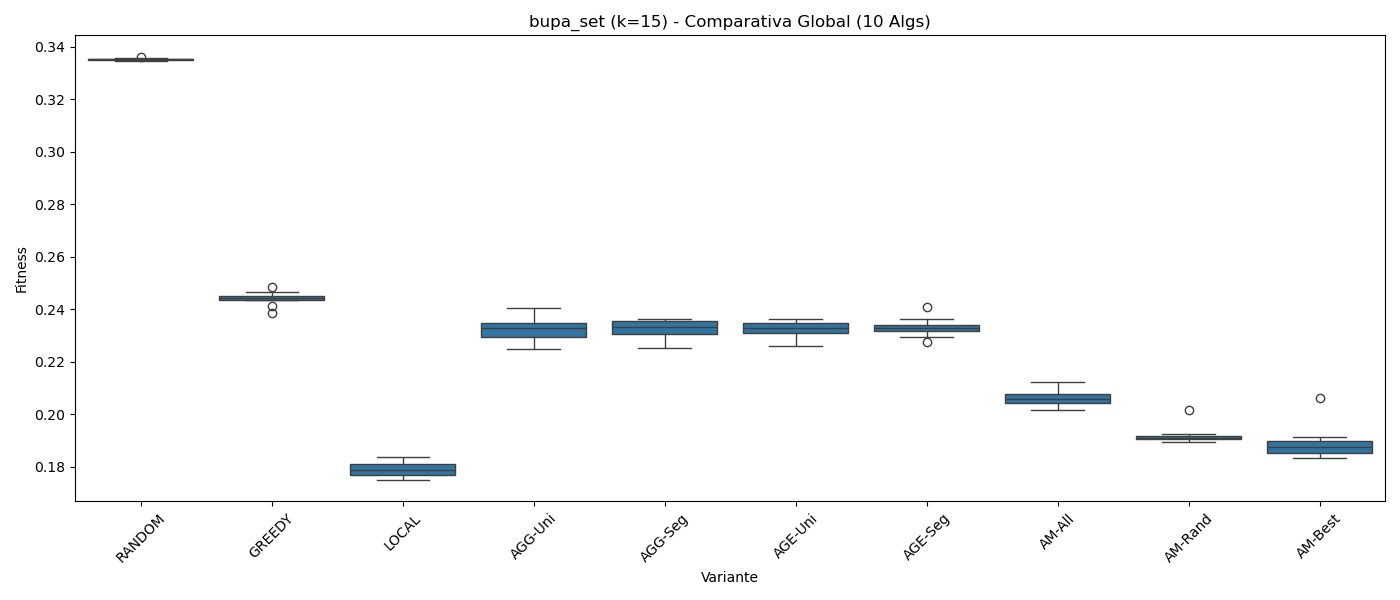
\includegraphics[width=0.495\textwidth]{../softwareP2/graficas/bupa_set_k15_all.png}
	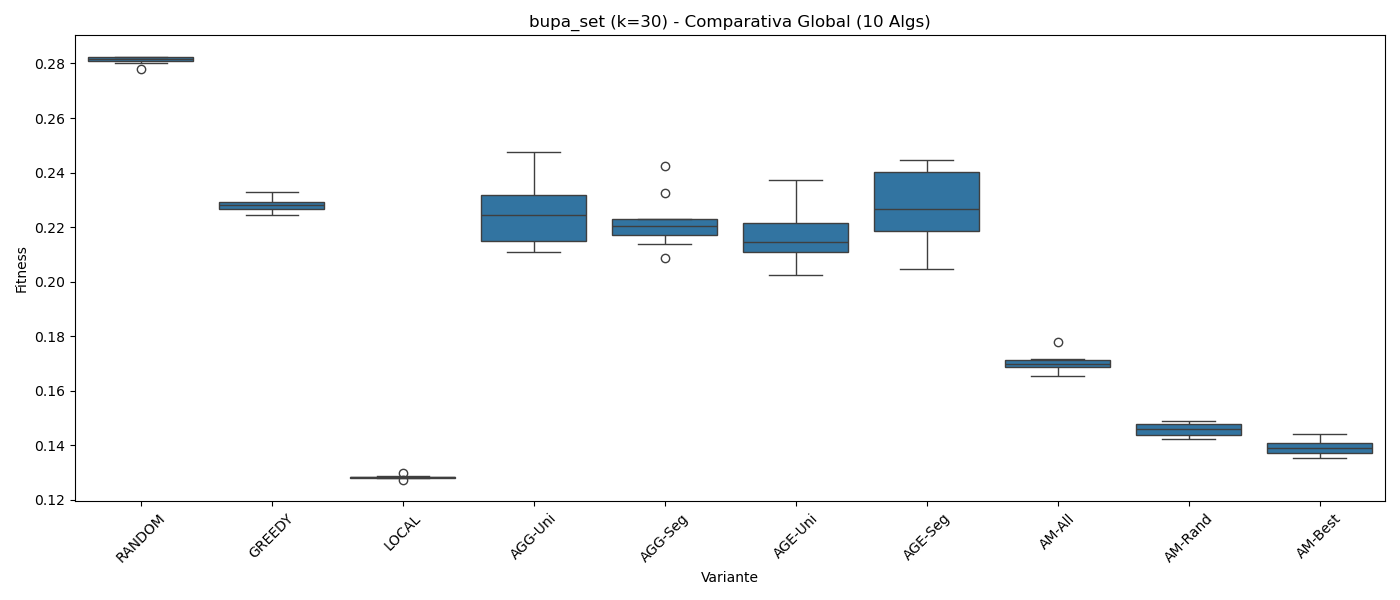
\includegraphics[width=0.495\textwidth]{../softwareP2/graficas/bupa_set_k30_all.png}
	\vspace{-20pt}
	\caption{\small Distribución del fitness para el dataset \textit{Bupa} con $k=15$ (izq) y $k=30$ (dcha)}
	\label{fig:bupa_var}
\end{figure}


Para $k=15$, \textit{Random} presenta claramente los peores resultados, seguido de \textit{Greedy}, mientras que \textit{Local} alcanza los mejores valores de \textit{fitness} con muy baja variabilidad. Los algoritmos genéticos (\texttt{AGG} y \texttt{AGE}) quedan en una posición intermedia muy compacta, todos alrededor de $\sim 0.233$ con baja dispersión, y los meméticos mejoran estos resultados, destacando \texttt{AM-Best} y \texttt{AM-Rand}, como puede verse claramente en la comparativa global.

Este comportamiento se aprecia con mayor detalle en la Figura \ref{fig:bupa_evolucion}. Para $k=15$, las cuatro variantes genéticas son prácticamente indistinguibles, con medianas entre $0.232$ y $0.234$ y cajas muy estrechas, lo que indica una convergencia homogénea independientemente del operador de cruce o esquema evolutivo. Para $k=30$, emergen diferencias más claras: \texttt{AGE-UN} obtiene la mejor mediana ($\sim 0.215$) y \texttt{AGE-Seg} presenta la mayor variabilidad y peores resultados, lo que sugiere que el cruce por segmento fijo no se adapta bien al mayor espacio de búsqueda en el esquema estacionario.

\begin{figure}[H]
	\centering
	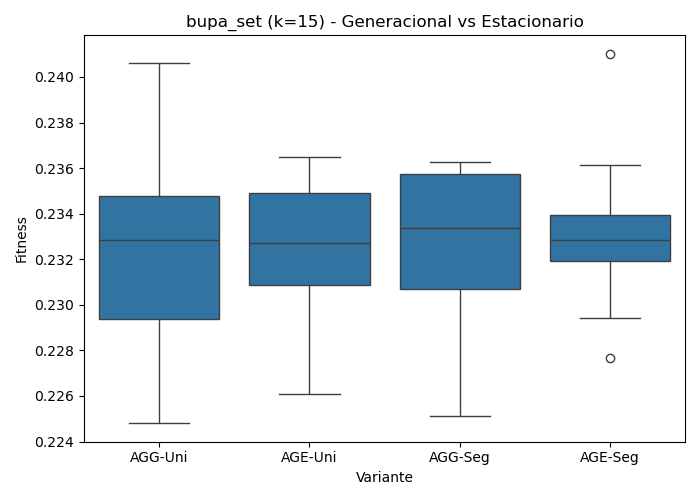
\includegraphics[width=0.495\textwidth]{../softwareP2/graficas/bupa_set_k15_evolution.png}
	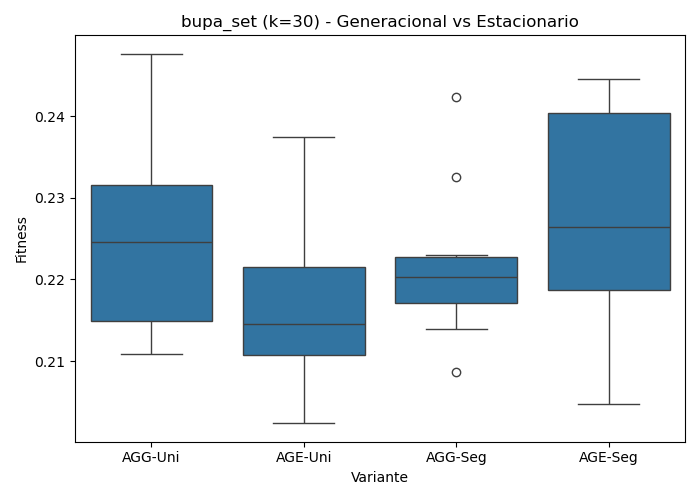
\includegraphics[width=0.495\textwidth]{../softwareP2/graficas/bupa_set_k30_evolution.png}
	\vspace{-20pt}
	\caption{\small Comparativa Generacional vs Estacionario para el dataset \textit{Bupa} con $k=15$ (izq) y $k=30$ (dcha)}
	\label{fig:bupa_evolucion}
\end{figure}


Finalmente, en la Figura \ref{fig:bupa_mem}, como puede observarse, se distinguen claramente las diferencias entre estrategias meméticas y la búsqueda Local.

\begin{figure}[H]
	\centering
	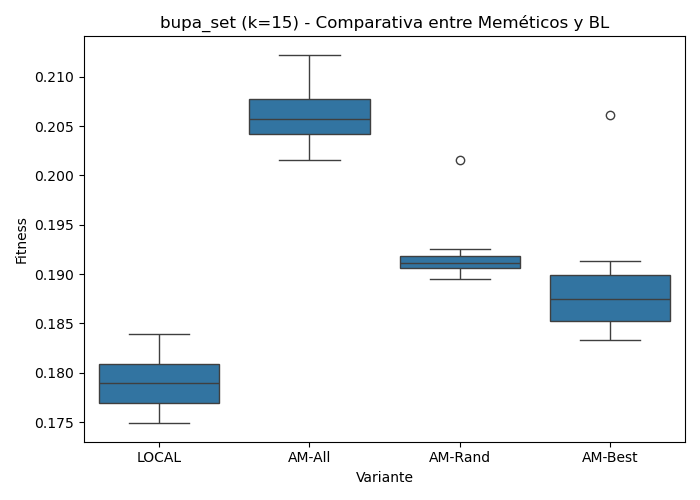
\includegraphics[width=0.495\textwidth]{../softwareP2/graficas/bupa_set_k15_zoom_mem.png}
	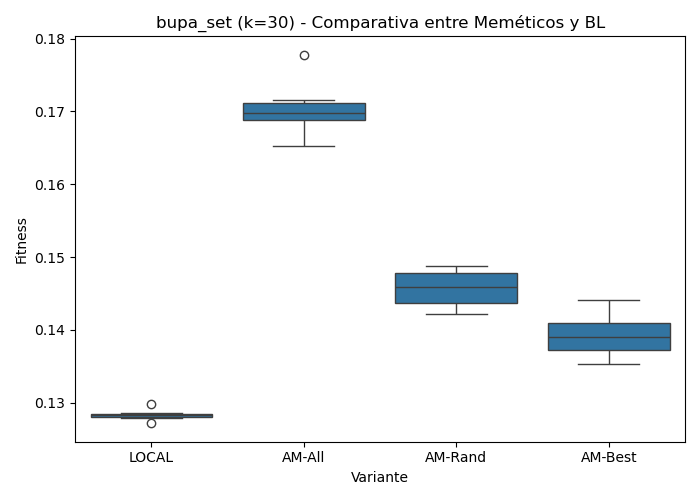
\includegraphics[width=0.495\textwidth]{../softwareP2/graficas/bupa_set_k30_zoom_mem.png}
	\vspace{-20pt}
	\caption{\small Comparativa entre Meméticos y Búsqueda Local para el dataset \textit{Bupa} con $k=15$ (izq) y $k=30$ (dcha)}
	\label{fig:bupa_mem}
\end{figure}

Para $k=15$, \textit{Local} sigue siendo el algoritmo más competitivo ($\sim 0.179$), lo que indica que con este dataset y valor de $k$ la exploración poblacional no compensa frente a una búsqueda local pura con el mismo presupuesto. \texttt{AM-Best} ($\sim 0.188$) y \texttt{AM-Rand} ($\sim 0.191$) se aproximan a \textit{Local}, mientras que \texttt{AM-All} queda más rezagado ($\sim 0.206$).

Para $k=30$, la brecha con 
\textit{Local} ($\sim 0.128$) se amplía: \texttt{AM-Best} ($\sim 0.139$) y \texttt{AM-Rand} ($\sim 0.146$) son los más cercanos, mientras que \texttt{AM-All} ($\sim 0.170$) queda muy por detrás. 

En conjunto, como se observa en todas las figuras, los algoritmos más intensivos en explotación (\textit{Local} y meméticos) no solo logran mejores resultados, sino que también presentan menor variabilidad, evidenciando una convergencia más robusta.

%%% GLASS
\paragraph{Dataset \texttt{glass\_set}}
\noindent En la Figura \ref{fig:glass_var} se muestra la distribución del \textit{fitness} para las distintas variantes de algoritmos evaluadas, considerando $k=15$ y $k=30$.

\begin{figure}[H]
	\centering
	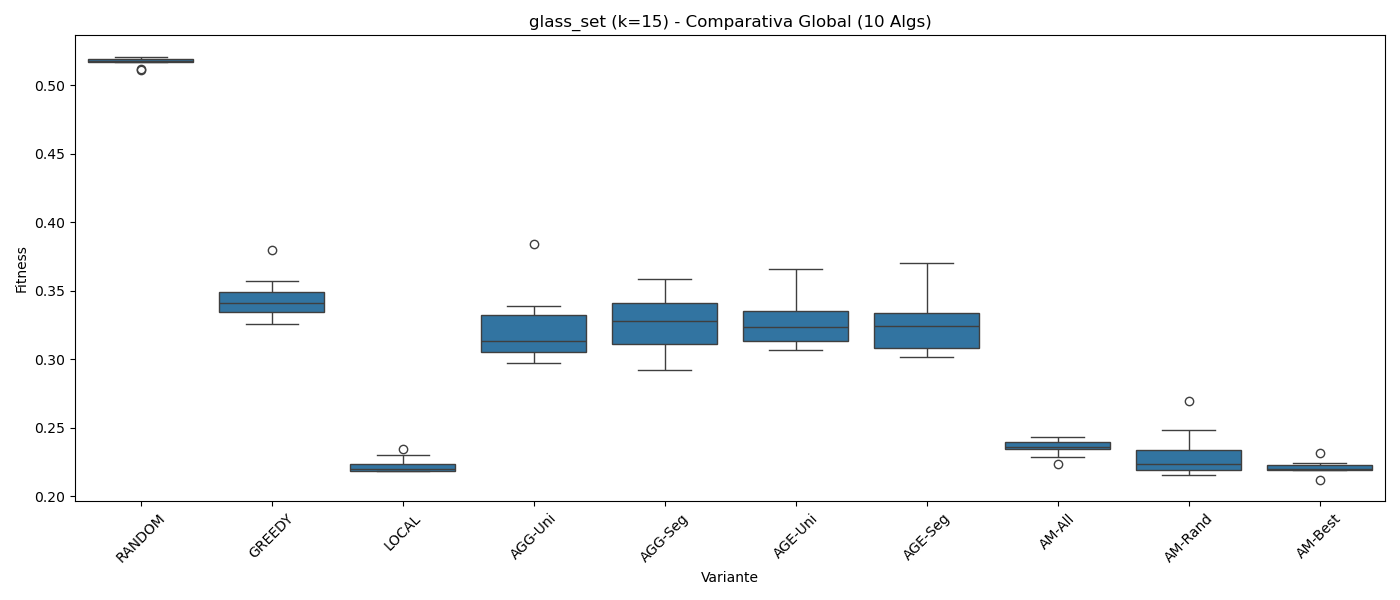
\includegraphics[width=0.495\textwidth]{../softwareP2/graficas/glass_set_k15_all.png}
	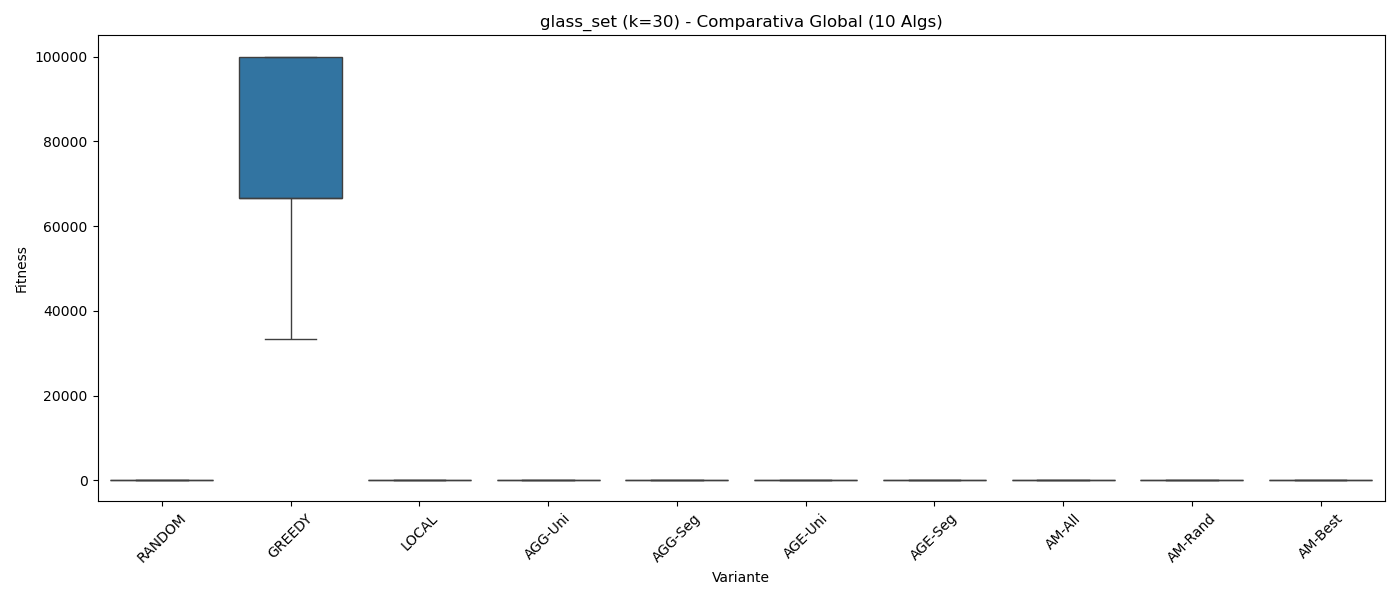
\includegraphics[width=0.495\textwidth]{../softwareP2/graficas/glass_set_k30_all.png}
	\vspace{-20pt}
	\caption{\small Distribución del fitness para el dataset \textit{Glass} con $k=15$ (izq) y $k=30$ (dcha)}
	\label{fig:glass_var}
\end{figure}

Para $k=15$, el comportamiento general es muy parecido al anterior: \textit{Random} presenta los peores resultados, seguido de \textit{Greedy} y \textit{Local} alcanza valores competitivos con baja dispersión. Los algoritmos genéticos (\texttt{AGG} y \texttt{AGE}) se sitúan en una franja intermedia entre $0.31$ y $0.33$, con \texttt{AGG-UN} mostrando la menor dispersión, mientras que los meméticos mejoran notablemente estos resultados, siendo \texttt{AM-Best} y \texttt{AM-Rand} los más destacados, con valores próximos a \textit{Local}.

Para $k=30$, la gráfica global presenta un comportamiento anómalo en \textit{Greedy}, cuyo \textit{fitness} alcanza valores muy altos, muy por encima del resto, debido a las penalizaciones por clusters vacíos. El resto de algoritmos, al explorar el espacio de búsqueda más ampliamente, evitan estas soluciones y se concentran en una franja de fitness más cercana a $0$, lo que distorsiona la escala visual de la comparativa global.

En la Figura \ref{fig:glass_genvsmem} se aprecia la comparativa entre genéticos y meméticos: los meméticos se separan claramente de los genéticos puros, con \texttt{AM-Best} ($\sim 0.153$) y \texttt{AM-Rand} ($\sim 0.160$) muy por debajo de cualquier variante genética ($0.265$--$0.320$).

\begin{figure}[H]
	\centering
	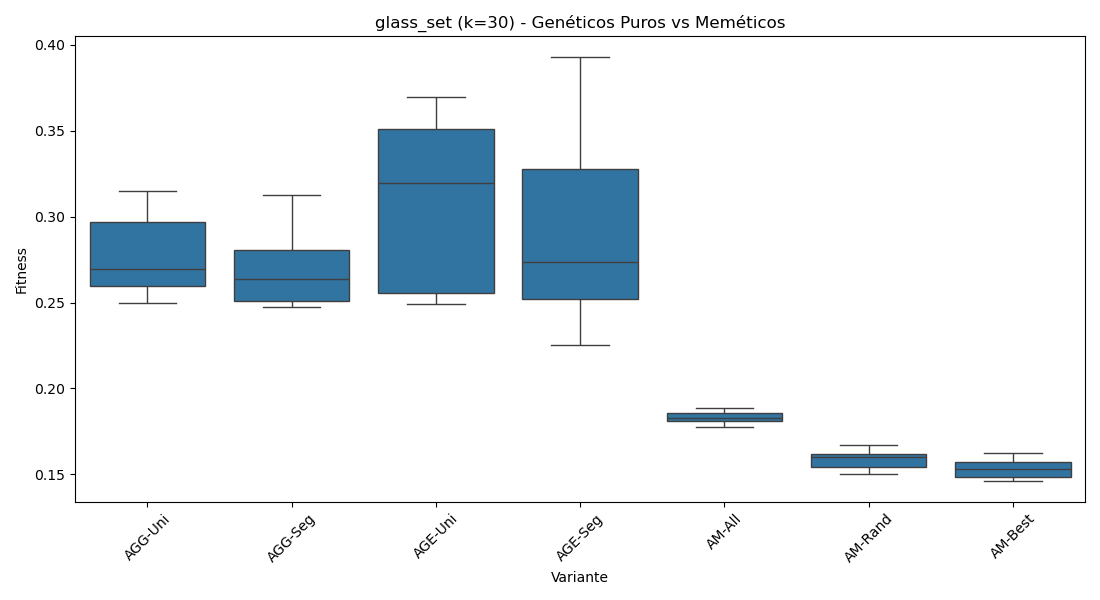
\includegraphics[width=0.55\textwidth]{../softwareP2/graficas/glass_set_k30_gen_vs_mem.png}
	\vspace{-20pt}
	\caption{\small Genéticos Puros vs Meméticos para el dataset \textit{Glass} con $k=15$ (izq) y $k=30$ (dcha)}
	\label{fig:glass_genvsmem}
\end{figure}

Para $k=15$, \texttt{AGG-UN} destaca con la mediana más baja ($\sim 0.312$) y menor dispersión, mientras que \texttt{AGG-Seg} presenta la mayor variabilidad. Para $k=30$, \texttt{AGG-Seg} obtiene ahora la mejor mediana ($\sim 0.263$) con poca dispersión, mientras que \texttt{AGE-UN} muestra la mayor variabilidad y peores resultados ($\sim 0.320$), evidenciando que el esquema estacionario con cruce uniforme es especialmente inestable al aumentar $k$. Esto lo comprobamos mejor en la Figura \eqref{fig:glass_evolucion}.

\begin{figure}[H]
	\centering
	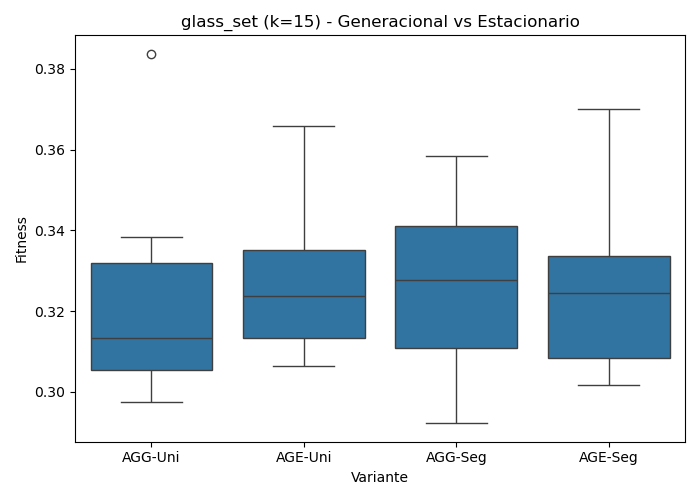
\includegraphics[width=0.495\textwidth]{../softwareP2/graficas/glass_set_k15_evolution.png}
	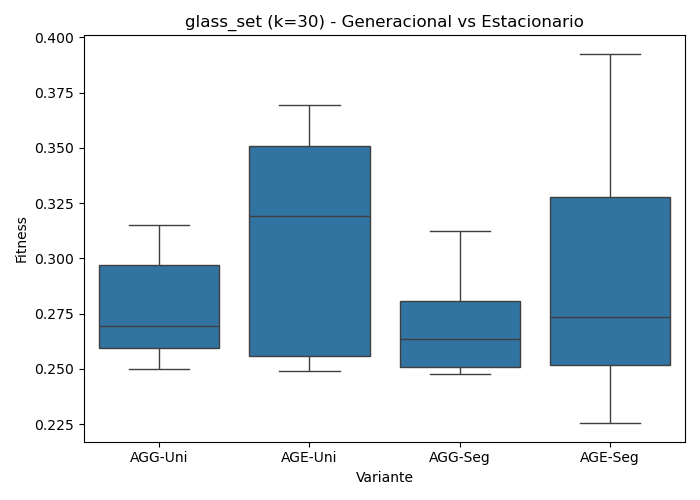
\includegraphics[width=0.495\textwidth]{../softwareP2/graficas/glass_set_k30_evolution.png}
	\vspace{-20pt}
	\caption{\small Comparativa Generacional vs Estacionario para el dataset \textit{Glass} con $k=15$ (izq) y $k=30$ (dcha)}
	\label{fig:glass_evolucion}
\end{figure}

Finalmente, la Figura \ref{fig:glass_mem} detalla la comparativa entre estrategias meméticas y BL.

\begin{figure}[H]
	\centering
	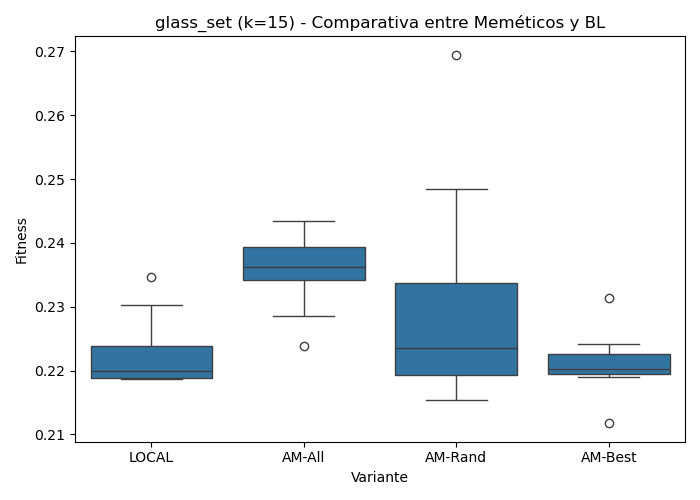
\includegraphics[width=0.495\textwidth]{../softwareP2/graficas/glass_set_k15_zoom_mem.png}
	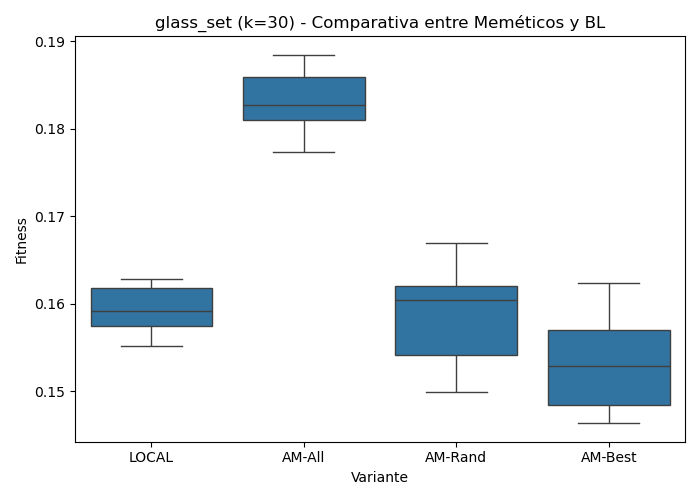
\includegraphics[width=0.495\textwidth]{../softwareP2/graficas/glass_set_k30_zoom_mem.png}
	\vspace{-20pt}
	\caption{\small Comparativa entre Meméticos y BL para el dataset \textit{Glass} con $k=15$ (izq) y $k=30$ (dcha)}
	\label{fig:glass_mem}
\end{figure}

En ambos valores de $k$ se repite el mismo patrón entre meméticos: \texttt{AM-Best} obtiene los mejores resultados, seguido de \texttt{AM-Rand}, mientras que \texttt{AM-All} presenta el peor rendimiento. La razón es estructural: \texttt{AM-All} distribuye las 100 evaluaciones de BLS entre los 50 individuos, de modo que cada uno recibe apenas 2 evaluaciones de media, una intensificación insuficiente. \texttt{AM-Best} concentra esas mismas evaluaciones en los 5 mejores individuos, que parten ya de regiones prometedoras del espacio de búsqueda.

Para $k=15$, \texttt{AM-Best} ($\sim 0.221$) y \textit{Local} ($\sim 0.221$) son prácticamente equivalentes en mediana, aunque \texttt{AM-Best} presenta menor dispersión. \texttt{AM-Rand} muestra una varianza muy elevada, con algunos outliers próximos a $0.27$, lo que indica inestabilidad en su selección aleatoria. \texttt{AM-All} ($\sim 0.236$) queda claramente por detrás. 

Para $k=30$, la ventaja de los meméticos selectivos se consolida: \texttt{AM-Best} ($\sim 0.153$) supera a \textit{Local} ($\sim 0.160$) y \texttt{AM-Rand} ($\sim 0.159$) se sitúa a un nivel similar, mientras que \texttt{AM-All} ($\sim 0.183$) sigue siendo el peor entre los meméticos. La diversidad genética resulta decisiva para $k=30$, donde el espacio de búsqueda es suficientemente grande como para que la BL pura quede atrapada en óptimos locales de menor calidad.

%%% ZOO
\paragraph{Dataset \texttt{zoo\_set}}
\noindent En la Figura \ref{fig:zoo_var} se muestra la distribución del \textit{fitness} para las distintas variantes de algoritmos evaluadas, considerando $k=15$ y $k=30$.

\begin{figure}[H]
	\centering
	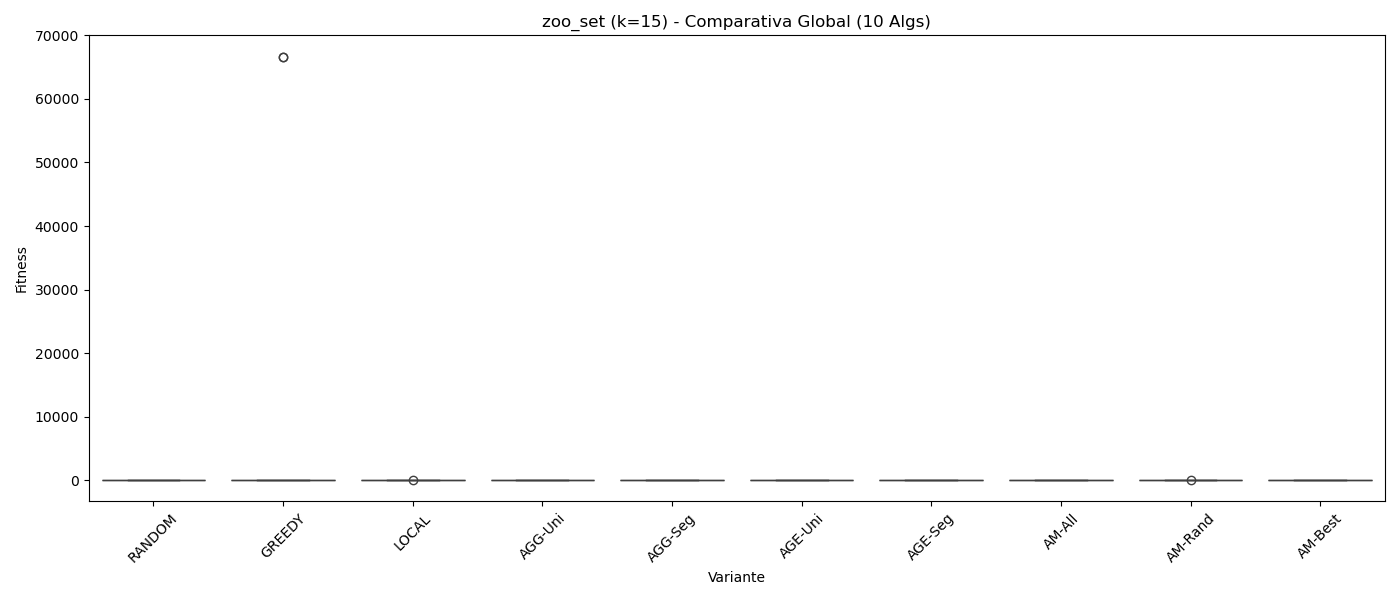
\includegraphics[width=0.495\textwidth]{../softwareP2/graficas/zoo_set_k15_all.png}
	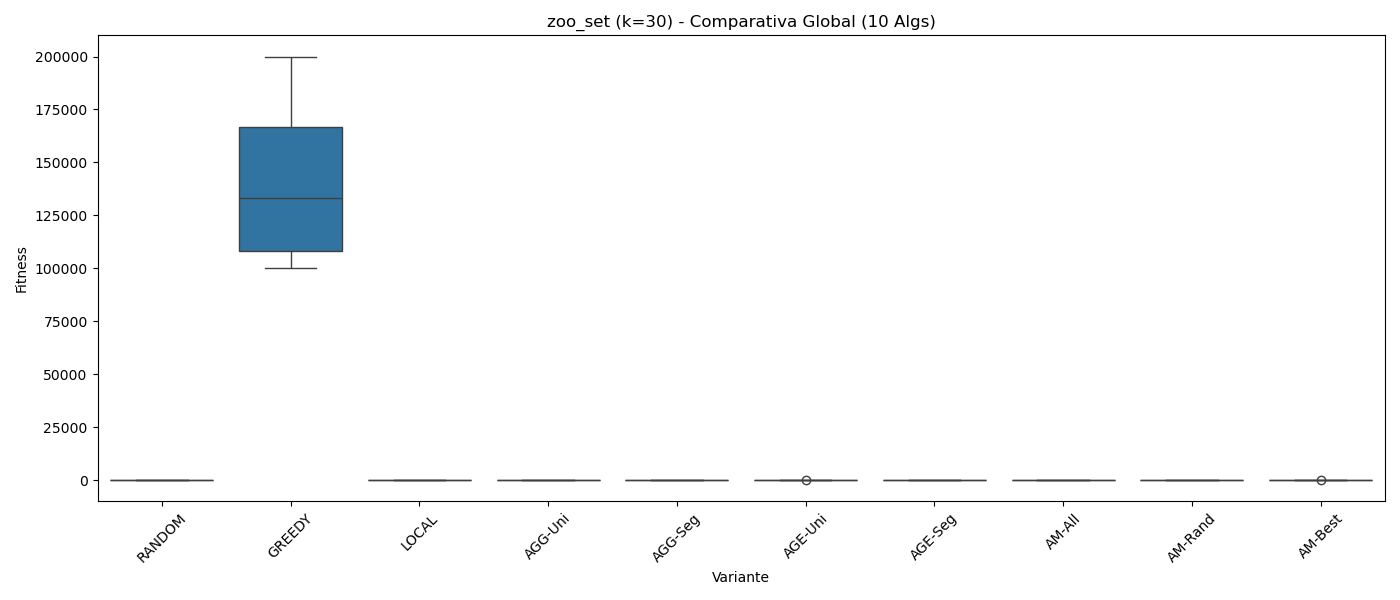
\includegraphics[width=0.495\textwidth]{../softwareP2/graficas/zoo_set_k30_all.png}
	\vspace{-20pt}
	\caption{\small Distribución del fitness para el dataset \textit{Zoo} con $k=15$ (izq) y $k=30$ (dcha)}
	\label{fig:zoo_var}
\end{figure}

Volvemos a observar lo que ocurría antes en \textit{glass\_set}, y es que en ambos valores de $k$, el comportamiento de \textit{Greedy} con sus altas penalizaciones por clusters vacíos lo lleva a presentar valores de \textit{fitness} muy altos, muy por encima del resto de algoritmos. Por ello, se incluyen figuras adicionales con zoom que permiten comparar en detalle las variantes genéticas entre sí y frente a los meméticos.

La Figura \ref{fig:zoo_gen_vs_mem} muestra la comparativa entre genéticos puros y meméticos, donde la ventaja de incorporar búsqueda local resulta especialmente evidente.

\begin{figure}[H]
	\centering
	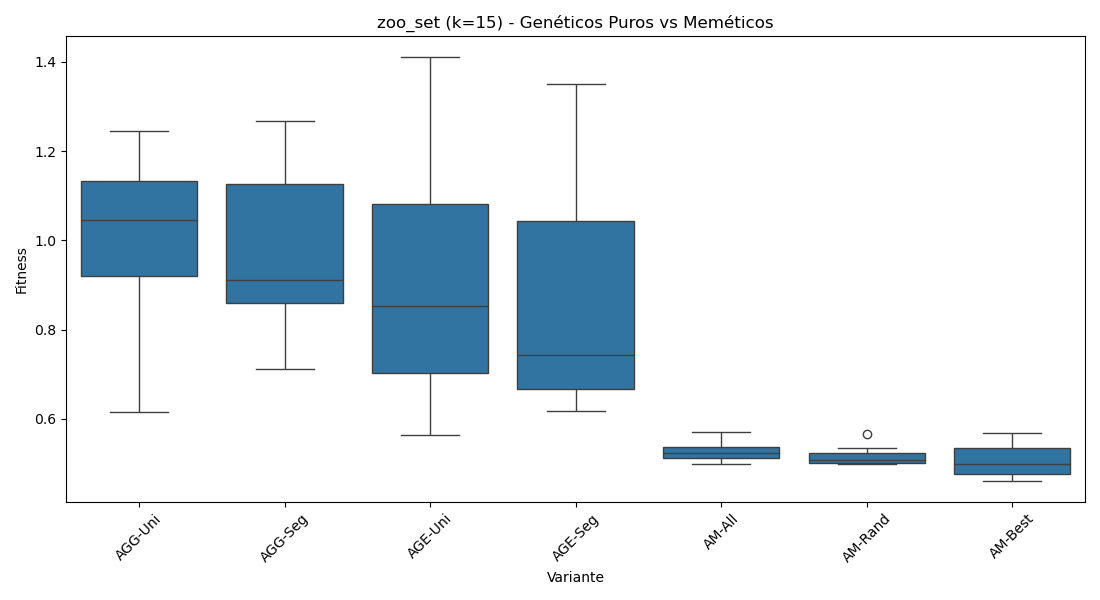
\includegraphics[width=0.495\textwidth]{../softwareP2/graficas/zoo_set_k15_gen_vs_mem.png}
	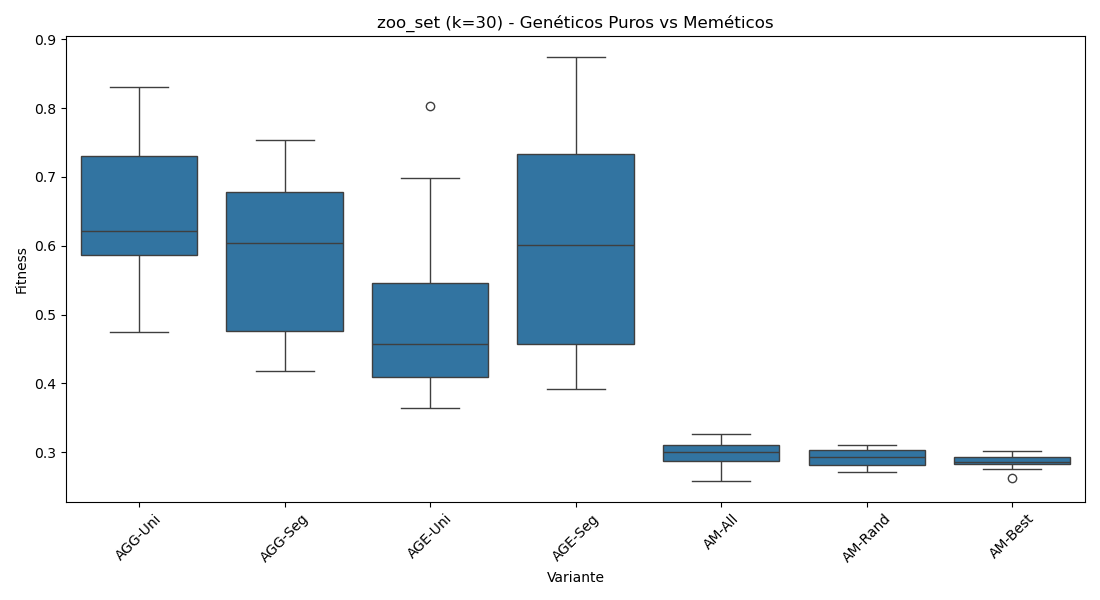
\includegraphics[width=0.495\textwidth]{../softwareP2/graficas/zoo_set_k30_gen_vs_mem.png}
	\vspace{-20pt}
	\caption{\small Genéticos Puros vs Meméticos para el dataset \textit{Zoo} con $k=15$ (izq) y $k=30$ (dcha)}
	\label{fig:zoo_gen_vs_mem}
\end{figure}

La mejora introducida por la hibridación con búsqueda local es notable en ambos valores de $k$. Para $k=15$, los genéticos puros se concentran en una franja elevada de $0.62$--$1.15$, mientras que los meméticos descienden fuertemente hasta $0.49$--$0.54$, una reducción de más del 10\% en \textit{fitness}. Para $k=30$, la separación es aún más pronunciada: los genéticos puros oscilan entre $0.45$ y $0.75$, mientras que los meméticos alcanzan valores muy cometitivos de $0.27$--$0.30$. En ambos casos, \texttt{AM-Best} es el que mayor beneficio obtiene de la intensificación local.

En la Figura \ref{fig:zoo_evolucion} se comparan exclusivamente las variantes genéticas.

Para $k=15$, las cuatro variantes genéticas presentan diferencias notables: los enfoques estacionarios (\texttt{AGE-UN} y \texttt{AGE-SF}) logran mejores resultados que los generacionales, situando sus medianas en torno a $0.85$--$0.90$. Para $k=30$, \texttt{AGE-UN} destaca claramente como la mejor opción pura, presentando la mediana más baja ($\sim 0.50$) y la menor dispersión. En contraste, las variantes generacionales (\texttt{AGG}) sufren más para optimizar este escenario, sugiriendo que la sustitución paulatina de la población del modelo estacionario preserva mejor las estructuras válidas en este conjunto de datos.

\begin{figure}[H]
	\centering
	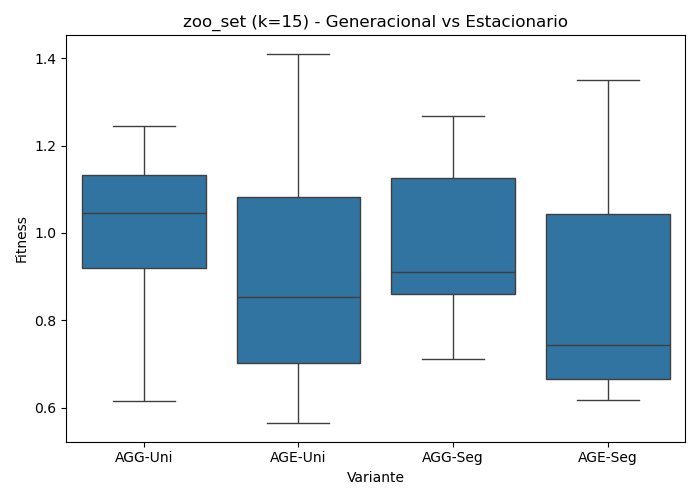
\includegraphics[width=0.495\textwidth]{../softwareP2/graficas/zoo_set_k15_evolution.png}
	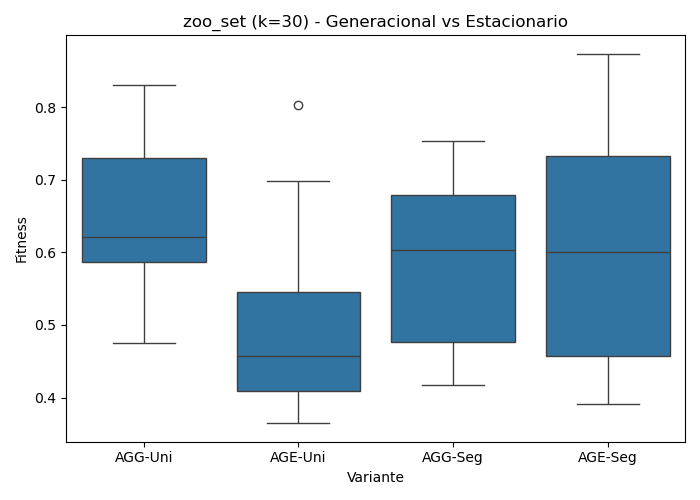
\includegraphics[width=0.495\textwidth]{../softwareP2/graficas/zoo_set_k30_evolution.png}
	\vspace{-20pt}
	\caption{\small Comparativa Generacional vs Estacionario para el dataset \textit{Zoo} con $k=15$ (izq) y $k=30$ (dcha)}
	\label{fig:zoo_evolucion}
\end{figure}

Finalmente, la Figura \ref{fig:zoo_mem} detalla la comparativa entre estrategias meméticas.

\begin{figure}[H]
	\centering
	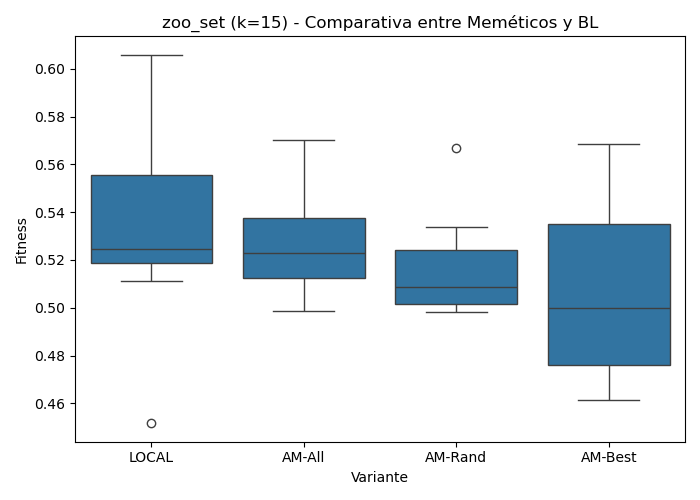
\includegraphics[width=0.495\textwidth]{../softwareP2/graficas/zoo_set_k15_zoom_mem.png}
	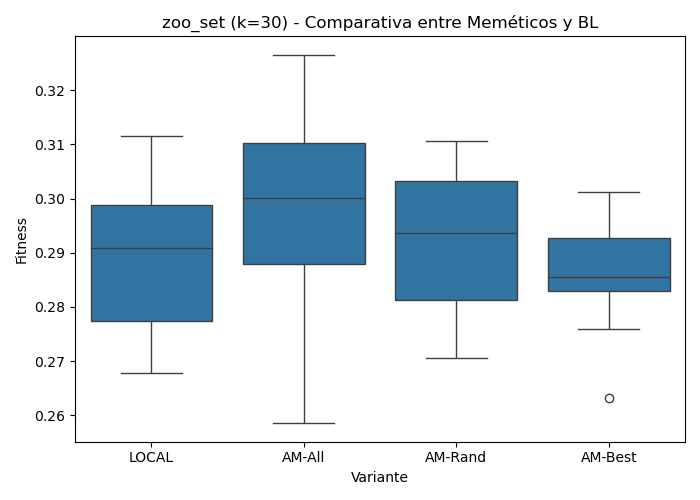
\includegraphics[width=0.495\textwidth]{../softwareP2/graficas/zoo_set_k30_zoom_mem.png}
	\vspace{-20pt}
	\caption{\small Comparativa entre Meméticos y BL para el dataset \textit{Zoo} con $k=15$ (izq) y $k=30$ (dcha)}
	\label{fig:zoo_mem}
\end{figure}

Para $k=15$, \texttt{AM-Best} logra la mejor mediana global (en torno a $0.49$), superando claramente a la Búsqueda Local (\textit{Local}, $\sim 0.53$) en la calidad central de las soluciones. Sin embargo, al observar la dispersión, destaca que \texttt{AM-Best} presenta una varianza notablemente mayor. Esto indica que la hibridación selectiva permite al algoritmo alcanzar las regiones más óptimas del espacio de búsqueda (como demuestran sus mejores valores), pero el resultado final fluctúa más dependiendo de las condiciones iniciales (semilla). Por el contrario, \textit{Local} presenta una menor varianza, lo que refleja un comportamiento muy estable pero indeseado: se estanca de forma consistente en óptimos locales de peor calidad. Las variantes \texttt{AM-Rand} y \texttt{AM-All} se sitúan en un punto intermedio, compactando la varianza pero con medianas ligeramente menos competitivas que \texttt{AM-Best}.

Para $k=30$, pasa algo bastante interesante: la Búsqueda Local pura (\textit{Local}) consigue la mejor mediana, superando un poco a los algoritmos meméticos. Esto significa que, en promedio, suele encontrar soluciones ligeramente mejores. Esto ocurre porque, en un espacio tan limitado como Zoo, la Búsqueda Local puede centrarse totalmente en mejorar una solución y exprimir al máximo cada zona (óptimos locales).

Por su parte, el algoritmo \texttt{AM-Best} destaca porque sus resultados son mucho más estables (tiene menos variabilidad). Aunque su mediana es un poco peor, casi siempre obtiene soluciones parecidas y bastante buenas. Esto pasa porque, en los meméticos, el cruce introduce cambios que a veces rompen estructuras que ya estaban bien optimizadas, lo que perjudica un poco el resultado final.


\subsubsection{Eficiencia computacional y tiempos de ejecución}

\noindent Un aspecto adicional que merece ser analizado es la eficiencia temporal de los algoritmos poblacionales. Observando la columna de tiempos de ejecución en las tablas, surge un patrón interesante: a pesar de que los algoritmos meméticos incorporan una fase de intensificación (Búsqueda Local Suave) que a priori podría intuirse como un cuello de botella, sus tiempos totales de cómputo resultan ser prácticamente idénticos a los de los algoritmos genéticos puros.

Por ejemplo, en el conjunto de datos \textit{Bupa} con $k=30$ (Cuadro \ref{tab_bupa30}), el algoritmo genético puro \texttt{AGG-UN} requiere una media de $29.46$ segundos, mientras que la variante memética \texttt{AM-Best} finaliza en $29.32$ segundos. Esta paridad temporal sugiere que el coste de consumir evaluaciones mediante saltos generacionales (lo que implica un gran sobrecoste en creación de descendencia, cruce, mutación y, sobre todo, ejecución constante del mecanismo de reparación de infactibilidades para toda la población) es computacionalmente equiparable a invertir esas mismas evaluaciones evaluando vecinos en la Búsqueda Local Suave (la cual modifica un único gen sin necesidad de recrear estructuras completas).

Por lo tanto, la verdadera fortaleza de las variantes meméticas (especialmente \texttt{AM-Best} y \texttt{AM-Rand}) en esta experimentación no reside en la reducción del tiempo bruto de ejecución, sino en la \textit{rentabilidad} de la optimización. Al obtener resultados de \textit{fitness} significativamente mejores e incuestionablemente superiores a nivel estadístico (por ejemplo, reduciendo el \textit{fitness} medio de $0.22$ a $0.14$ en el citado caso de \textit{Bupa} $k=30$) consumiendo exactamente el mismo presupuesto temporal de CPU, la hibridación demuestra ser una arquitectura computacionalmente mucho más eficiente.


\subsubsection{Conclusiones generales del análisis}

\noindent A modo de síntesis, la experimentación y el análisis visual confirman que la hibridación algorítmica representa la estrategia más robusta y eficaz para abordar este problema de \textit{clustering} con restricciones. Mientras que los algoritmos de trayectoria simple muestran problemas de convergencia prematura o incapacidad para reparar soluciones infactibles (como evidencia el estancamiento de \textit{Greedy}), y los genéticos puros adolecen de falta de intensificación local, los Algoritmos Meméticos logran el equilibrio óptimo entre exploración y explotación. 

En particular, la variante \texttt{AM-Best} se erige de forma unánime como la arquitectura superior del estudio. La aplicación selectiva de la Búsqueda Local Suave al $10\%$ de la población no solo reporta sistemáticamente los mejores valores de \textit{fitness} y sortea con mayor éxito las topologías más complejas ($k=30$), sino que además lo hace invirtiendo exactamente el mismo presupuesto temporal, demostrando que optimizar a los mejores individuos es una táctica altamente rentable, computacionalmente eficiente y estadísticamente significativa.

\vspace{0.4cm}
\noindent \textbf{Nota:} Para dotar de rigor formal a estas conclusiones empíricas y confirmar que la superioridad de la arquitectura memética no es fruto del azar, a continuación se detalla el análisis estadístico realizado mediante el test no paramétrico de Wilcoxon.

%%%%%%%%%%%%%%%%%%%%%%%%%%%%%%%%%%%%%%%%%%%%%%%%%%%%%%%%%%%%%%%%%%
\newpage
\section{Contraste de Hipótesis mediante el Test de Wilcoxon}

\noindent A lo largo del análisis previo, tanto la inspección visual de las gráficas como los valores promedio han sugerido una clara superioridad de los Algoritmos Meméticos frente a los Algoritmos Genéticos puros. No obstante, con el fin de dotar a esta afirmación de mayor rigor estadístico y justificar la inclusión de la Búsqueda Local en el esquema evolutivo, se ha realizado un contraste de hipótesis emparejado entre el algoritmo generacional puro (\texttt{AGG-UN}) y la mejor variante memética (\texttt{AM-Best}).

Dado que ambos algoritmos han sido evaluados bajo condiciones estrictamente emparejadas (utilizando las mismas $10$ semillas aleatorias en cada experimento) y que no puede asumirse \textit{a priori} la normalidad de las distribuciones del \textit{fitness}, no resulta apropiado aplicar un test paramétrico como el test de Student. En su lugar, se ha empleado el \textbf{test de los rangos signados de Wilcoxon}, un test no paramétrico idóneo para estas condiciones.

Las hipótesis consideradas en el estudio son:
\begin{itemize}
	\item \textbf{Hipótesis nula ($H_0$):} No existen diferencias significativas entre las medianas del \textit{fitness} obtenido por el algoritmo genético \texttt{AGG-UN} y el algoritmo memético \texttt{AM-Best}.
	\item \textbf{Hipótesis alternativa ($H_1$):} El algoritmo memético \texttt{AM-Best} obtiene valores de \textit{fitness} significativamente menores (mejores) que el algoritmo genético \texttt{AGG-UN}.
\end{itemize}

Para la realización del contraste se ha desarrollado un \textit{script} en Python utilizando la librería \texttt{scipy.stats}. El test se ha aplicado de forma independiente para cada conjunto de datos (\textit{Bupa, Glass, Zoo}) y para cada valor de $k$ ($15$ y $30$), fijando un nivel de significación $\alpha = 0.05$. Los resultados obtenidos son los siguientes:

\begin{verbatim}
RESULTADOS DEL TEST DE WILCOXON (AGG-Uniform vs AM-Best)
------------------------------------------------------------
Dataset: data/bupa_set   | k: 15 | p-valor: 9.766e-04
Diferencia significativa (AM-Best es estadísticamente mejor)

Dataset: data/bupa_set   | k: 30 | p-valor: 9.766e-04
Diferencia significativa (AM-Best es estadísticamente mejor)

Dataset: data/glass_set  | k: 15 | p-valor: 9.766e-04
Diferencia significativa (AM-Best es estadísticamente mejor)

Dataset: data/glass_set  | k: 30 | p-valor: 9.766e-04
Diferencia significativa (AM-Best es estadísticamente mejor)

Dataset: data/zoo_set    | k: 15 | p-valor: 9.766e-04
Diferencia significativa (AM-Best es estadísticamente mejor)

Dataset: data/zoo_set    | k: 30 | p-valor: 9.766e-04
Diferencia significativa (AM-Best es estadísticamente mejor)
\end{verbatim}

\subsubsection*{Interpretación y conclusiones del contraste}

\noindent En todos los escenarios analizados, los \textit{p-valores} obtenidos mediante el test de Wilcoxon son claramente inferiores al nivel de significación establecido ($\alpha = 0.05$). Por tanto, los datos aportan evidencia estadística suficiente para rechazar la hipótesis nula ($H_0$) en favor de la hipótesis alternativa ($H_1$).

Un aspecto analítico interesante es la magnitud exacta de estos \textit{p-valores}. En los seis escenarios, el test arroja un valor de $9.766 \times 10^{-4}$. Este es el valor probabilístico mínimo posible para una muestra emparejada de tamaño $N=10$ ($1/2^{10} \approx 9.77 \times 10^{-4}$), lo que indica una dominancia absoluta: la variante \texttt{AM-Best} superó a \texttt{AGG-UN} en el 100\% de las semillas ejecutadas.

En definitiva, este contraste de hipótesis arroja un resultado concluyente: demuestra estadísticamente que la hibridación algorítmica es altamente efectiva en este problema. La incorporación de una Búsqueda Local Suave aplicada al 10\% de los mejores individuos de la población mejora sistemáticamente el proceso de optimización frente al uso exclusivo de los operadores de cruce y mutación tradicionales, justificando de manera rigurosa el desarrollo y adopción de arquitecturas meméticas.


%%%%%%%%%%%%%%%%%%%%%%%%%%%%%%%%%%%%%%%%%%%%%%%%%%%%%%%%%%%%%%%%%%%%%%%%%%%%%%%%%%%%%%%%%%%%%%%%%%%
\newpage
\section{Referencias y recursos utilizados}

Para la realización de esta práctica y la elaboración de la presente memoria, se han consultado y utilizado los siguientes recursos:

\begin{itemize}
	\item \textbf{Material de la asignatura:} Diapositivas, guión de prácticas y recursos de PRADO.
	
	\item \textbf{Herramientas de Inteligencia Artificial:} Se ha hecho uso de herramientas de IA generativa como apoyo en tareas de programación y redacción. En concreto, se han empleado para:
	\begin{itemize}
		\item Resolver dudas puntuales de sintaxis en C++ y mejorar la organización del archivo \texttt{Makefile}.
		\item Desarrollar el script de Python (\texttt{graf.py}), utilizando las librerías \texttt{pandas}, \texttt{matplotlib} y \texttt{seaborn}, para la generación automatizada de gráficos (\textit{boxplots}) y el procesamiento de los datos almacenados en archivos \texttt{.csv}.
		\item Asistir en el formateo, revisión y estructuración del documento final en \LaTeX.
	\end{itemize}
	
	\item Documentación oficial de C++ (\href{https://cppreference.com}{\textit{cppreference.com}}) para el manejo de estructuras de datos estándar, y documentación oficial de las librerías de Python empleadas para la visualización de datos.
	
	\item Para la realización del análisis estadístico de los resultados, en la aplicación del test de hipótesis de Wilcoxon, se ha utilizado el material de la asignatura \textit{Inferencia Estadística},  dentro de la parte de Matemáticas del doble grado.
\end{itemize}

%%%%%%%%%%%%%%%%%%%%%%%%%%%%%%%%%%%%%%%%%%%%%%%%%%%%%%%%%%%%%%%%%%%%%%%%%%%%%%%%%%%%%%%%%%%%%%%%%%%
\newpage
\section{Anexo - Falta de espacio}

\noindent\textbf{Mecanismo de Reparación (\texttt{repairSolution}):}
Todo individuo generado tras el cruce se somete a una verificación estricta. Si algún clúster queda vacío (0 instancias asignadas), el método busca instancias pertenecientes a clústeres sobrepoblados (con más de una instancia) y prueba a reasignarlas al clúster vacío. El proceso sigue estos pasos:

\begin{enumerate}
	\item Calcula la frecuencia de cada clúster en la solución.
	\item Para cada clúster $c$ sin elementos:
	\begin{itemize}
		\item Recopila índices de instancias que provienen de clústeres con al menos dos elementos.
		\item Mezcla el orden de esas instancias para evitar sesgos.
		\item Prueba secuencialmente: mueve la instancia al clúster vacío y evalúa la infactibilidad global mediante el método \texttt{calculateInfeasibilityDelta()}.
		\item Si el cambio $\Delta \leq 0$ (es decir, la infactibilidad no empeora), consolida el movimiento y pasa al siguiente clúster vacío. Esto permite mantener o mejorar la factibilidad sin necesidad de exigir infactibilidad global cero.
		\item En caso contrario, deshace el cambio y prueba con la siguiente instancia.
	\end{itemize}
	\item Si no se encuentra ninguna reasignación con $\Delta\leq0$, aplica un \textit{fallback} forzado con la primera instancia candidata (garantiza que no queden clústeres vacíos, aunque pueda generar infactibilidad temporal; esta será tratada por la función de penalización en el fitness).
\end{enumerate}

Este mecanismo asegura que la mayoría de las soluciones sean factibles en cuanto a cardinalidad de los clústeres, respetando al mismo tiempo las restricciones estructurales del problema.

A continuación, mostramos el pseudocódigo:

\begin{algorithm}
	\begin{algorithmic}
		\Function{RepairSolution}{sol}
		\State $k \leftarrow$ número de clusters
		\State $n \leftarrow$ longitud del cromosoma
		\State $contador \leftarrow$ vector de ceros de tamaño $k$
		
		\For{$i \leftarrow 0$ hasta $n-1$}
		\State $contador[sol[i]] \leftarrow contador[sol[i]] + 1$
		\EndFor
		
		\For{cada cluster $c$ desde $0$ hasta $k-1$}
		\If{$contador[c] = 0$}
		\State $robable \leftarrow$ lista vacía
		\For{$i \leftarrow 0$ hasta $n-1$}
		\If{$contador[sol[i]] > 1$}
		\State añadir $i$ a $robable$
		\EndIf
		\EndFor
		\State $robable \leftarrow$ \Call{shuffle}{$robable$}
		\State $reparado \leftarrow$ falso
		
		\For{cada $inst$ en $robable$}
		\State $old\_cluster \leftarrow sol[inst]$
		\State $delta \leftarrow$ \Call{calculateInfeasibilityDelta}{$sol, inst, old\_cluster, c$}
		\If{$delta \leq 0$}
		\State $contador[old\_cluster] \leftarrow contador[old\_cluster] - 1$
		\State $sol[inst] \leftarrow c$
		\State $contador[c] \leftarrow contador[c] + 1$
		\State $reparado \leftarrow$ verdadero
		\State \textbf{break}
		\EndIf
		\EndFor
		
		\If{$\neg reparado$ y $robable$ no vacía}
		\State $inst \leftarrow$ primera de $robable$
		\State $contador[sol[inst]] \leftarrow contador[sol[inst]] - 1$
		\State $sol[inst] \leftarrow c$
		\State $contador[c] \leftarrow contador[c] + 1$
		\EndIf
		\EndIf
		\EndFor
		\EndFunction
	\end{algorithmic}
\end{algorithm}


%%%%%%%%%%%%%%%%%%%%%%%%%%%%%%%%%%%%%%%%%%%%%%%%%%%%%%%%%%%%%%%%%%%%%%%%%%%%%%%%%%%%%%%%%%%%%%%%%%%



\end{document}